%%%%%%%%%%%%%%%%%%%%%%%%%%%%%%%%%%%%%%%%%%%%%%%%%%%%%%%%%%%%%%%%%%%%%%%%%%%%
% AGUtmpl.tex: this template file is for articles formatted with LaTeX2e,
% Modified July 2014
%
% This template includes commands and instructions
% given in the order necessary to produce a final output that will
% satisfy AGU requirements.
%
% PLEASE DO NOT USE YOUR OWN MACROS
% DO NOT USE \newcommand, \renewcommand, or \def.
%
% FOR FIGURES, DO NOT USE \psfrag or \subfigure.
%
%%%%%%%%%%%%%%%%%%%%%%%%%%%%%%%%%%%%%%%%%%%%%%%%%%%%%%%%%%%%%%%%%%%%%%%%%%%%
%
% All questions should be e-mailed to latex@agu.org.
%
%%%%%%%%%%%%%%%%%%%%%%%%%%%%%%%%%%%%%%%%%%%%%%%%%%%%%%%%%%%%%%%%%%%%%%%%%%%%
%
% Step 1: Set the \documentclass
%
% There are two options for article format: two column (default)
% and draft.
%
% PLEASE USE THE DRAFT OPTION TO SUBMIT YOUR PAPERS.
% The draft option produces double spaced output.
%
% Choose the journal abbreviation for the journal you are
% submitting to:

% jgrga JOURNAL OF GEOPHYSICAL RESEARCH
% gbc   GLOBAL BIOCHEMICAL CYCLES
% grl   GEOPHYSICAL RESEARCH LETTERS
% pal   PALEOCEANOGRAPHY
% ras   RADIO SCIENCE
% rog   REVIEWS OF GEOPHYSICS
% tec   TECTONICS
% wrr   WATER RESOURCES RESEARCH
% gc    GEOCHEMISTRY, GEOPHYSICS, GEOSYSTEMS
% sw    SPACE WEATHER
% ms    JAMES
% ef    EARTH'S FUTURE
% ea    EARTH AND SPACE SCIENCE
%
%
%
% (If you are submitting to a journal other than jgrga,
% substitute the initials of the journal for "jgrga" below.)

\documentclass[draft,grl]{agutex}   %draft, [ms]
% To create numbered lines:

% If you don't already have lineno.sty, you can download it from
% http://www.ctan.org/tex-archive/macros/latex/contrib/ednotes/
% (or search the internet for lineno.sty ctan), available at TeX Archive Network (CTAN).
% Take care that you always use the latest version.

% To activate the commands, uncomment \usepackage{lineno}
% and \linenumbers*[1]command, below:

\usepackage{lineno}

\linenumbers*[1]
%  To add line numbers to lines with equations:
%  \begin{linenomath*}
%  \begin{equation}
%  \end{equation}
%  \end{linenomath*}
%%%%%%%%%%%%%%%%%%%%%%%%%%%%%%%%%%%%%%%%%%%%%%%%%%%%%%%%%%%%%%%%%%%%%%%%%
\usepackage{url}
\usepackage{amsmath}
\usepackage{rotating} 

\usepackage{lineno}
\usepackage[bottom]{footmisc}

\usepackage{graphics}

%\usepackage[dvips]{graphicx}
 
\usepackage{color}
\definecolor{pinkred}{rgb}{1.0, 0.4, 0.4}

% Author names in capital letters:
\authorrunninghead{HUANG ET AL.}

% Shorter version of title entered in capital letters:
\titlerunninghead{}

%Corresponding author mailing address and e-mail address:
\authoraddr{Corresponding author: Xingying Huang,
Department of Land, Air and Water Resources, \\
 University of California Davis, Davis, CA 95616, USA.
 (xyhuang@ucdavis.edu)}
 
%Department of Hydrology and Water Resources, University of
%Arizona, Harshbarger Building 11, Tucson, AZ 85721, USA.
%(a.b.smith@hwr.arizona.edu)}

\begin{document}

%% ------------------------------------------------------------------------ %%
%
%  TITLE
%
%% ------------------------------------------------------------------------ %%


\title{The impacts of irrigation on California's climate modeled by the variable-resolution CESM}
%
% e.g., \title{Terrestrial ring current:
% Origin, formation, and decay $\alpha\beta\Gamma\Delta$}
%

%% ------------------------------------------------------------------------ %%
%
%  AUTHORS AND AFFILIATIONS
%
%% ------------------------------------------------------------------------ %%

%Use \author{\altaffilmark{}} and \altaffiltext{}

% \altaffilmark will produce footnote;
% matching \altaffiltext will appear at bottom of page.

% \authors{A. B. Smith,\altaffilmark{1}
% Eric Brown,\altaffilmark{1,2} Rick Williams,\altaffilmark{3}
% John B. McDougall\altaffilmark{4}, and S. Visconti\altaffilmark{5}}

%\altaffiltext{1}{Department of Hydrology and Water Resources,
%University of Arizona, Tucson, Arizona, USA.}

%\altaffiltext{2}{Department of Geography, Ohio State University,
%Columbus, Ohio, USA.}

%\altaffiltext{3}{Department of Space Sciences, University of
%Michigan, Ann Arbor, Michigan, USA.}

%\altaffiltext{4}{Division of Hydrologic Sciences, Desert Research
%Institute, Reno, Nevada, USA.}

    \authors{Xingying Huang,\altaffilmark{1}
  Paul A. Ullrich, \altaffilmark{1} }

\altaffiltext{1}{Department of Land, Air and Water Resources, University of California, Davis}


%%%%%%%%%%%%%%%%%%%%%%%%%%%%%%%%%%%%%%%%%%%%%%%%%%%%%%%%%%%%%%%%%%%%%
% ABSTRACT
%
% Enter your Abstract here

\begin{abstract}

The recently developed variable-resolution option within the Community Earth System Model (VR-CESM) is applied to study the irrigation effect on regional climate over Central Valley in California. The irrigation practice plays important role in regulating the climate patterns of heavily irrigated regions. A flexible irrigation scheme with relatively realistic estimates of regional agricultural water use is enabled for the land model of the CESM. We investigated the impact of irrigation not only on mean climatology, but also on heat extremes over the recent period from year 1980-01-01 to 2005-12-31 with the fine grid resolution at $0.25^\circ$ ($\sim$28 km). Simulation output from a control run without irrigation and two irrigation-enabled runs are analyzed, with gridded observations and weather station datasets. During the summer (when the irrigation peaks), cooling effect caused by irrigation is obvious for daily maximum near-surface temperature (Tmax) with magnitude around 1.3 K (seasonally averaged), under California's dry Mediterranean climate. The latent heat flux increased by 71$\%$ during the daytime mainly caused by raised evaporation from the surface. The specific humidity also increased by about 15$\%$, and the averaged soil moisture show a significant increase though with a slight amplitude ($\sim$5$\%$) under irrigation. The frequency distribution of Tmax is improved, and both length and frequency of hot spells are well captured with irrigation enabled. For cropland, the heat stress frequency reduced for about 34$\%$ under irrigation. 

%Tmin is scarcely affected by irrigation, and no notable difference is observed when reducing the irrigated water by half, which may due to that irrigated water does not effectively infiltrate into lower soil layers when reaching certain level. 
%This study adds the value of variable-resolution global climate models (VRGCMs) in capturing fine-scale land-air interactions for long-term climate and can motivate more realistic climate adaptation strategies.


\end{abstract}


\begin{article}


%%%%%%%%%%%%%%%%%%%%%%%%%%%%%%%%%%%%%%%%%%%%%%%%%%%%%%%%%%%%%%%%%%%%%
% MAIN BODY OF PAPER
%%%%%%%%%%%%%%%%%%%%%%%%%%%%%%%%%%%%%%%%%%%%%%%%%%%%%%%%%%%%%%%%%%%%%
%
\section{Introduction}

Over the past century, human activity has strongly impacted the climate both globally and regionally, largely through impacts associated with increasing greenhouse gases \citep{solomon2007climate}, but also as a result of land cover changes, particularly deforestation and urbanization \citep{bonan1997effects, pielke2002influence, kueppers2008seasonal}. Conversion of the natural land surface to cropland features prominently in this change, which is accompanied by modified albedo and changes to both sensible and latent heat fluxes \citep{foley2003green}. Additionally, besides changes to energy balance, land management also plays a important role in affecting the climate by modifying the carbon and water cycles, which are impacted by cropping length and irrigation strategy \citep{lobell2006biogeophysical}. The pronounced cooling effect by irrigation, especially over regions where irrigation is extensive, has also been emphasized by previous studies \citep{kueppers2007irrigation, lobell2008effect}.  


%In some areas with extensive irrigation, the cooling effect by irrigation can match or even exceed the impacts of greenhouse warming [Diffenbaugh, 2009; Kueppers et al., 2007; Lobell et al., 2008; Puma and Cook, 2010].
%The effect of irrigation on climate seems to be much more prominent than the land surface change (govindasamy2001land, bounoua2002effects, matthews2004natural). 

California is the most irrigated state in the US, and most of California's irrigated cropland is distributed over the Central Valley (CV), which is in turn responsible for 25$\%$ of the agricultural products in the U.S. \citep{wilkinson2002preparing}. The CV extends 600 km between its northernmost and southernmost point and is between 60-100km in width.  It features a vast agricultural industry, that has adapted to an extremely dry growing season within its Mediterranean climate, through the adoption of extensive irrigation practices. The USGS reports that in the year 2000, approximately 42 km$^3$ of water was used over $\sim$41,000 km$^2$ of irrigated area within California \citep{doll2002global, famiglietti2011satellites}. \cite{bonfils2007empirical} found that irrigation over CV has decreased summertime maximum temperature by $\sim$2-3 K in heavily-irrigated areas compared with nearby non-irrigated areas, based on long-term temperature records, although these impacts had a negligible effect on nighttime temperatures. Similar impacts have also been demonstrated in Nebraska's irrigated areas by \citet{mahmood2006impacts}.

%irrigated area (shiklomanov2000appraisal, siebert2005development).
%irrigated water and area for year 2000 http://pubs.usgs.gov/circ/2004/circ1268/htdocs/table07.html  http://pubs.usgs.gov/circ/2004/circ1268/htdocs/text-ir.html

%More than half of this area (CV) has been converted to agriculture since the presettlement period. The Central Valley produces one quarter of the agricultural products in the United States, with an annual income exceeding $26 billion and an export revenue exceeding $6.7 billion (wilkinson2002preparing). Thus, understanding the climate variability in this area is critical for projecting future economic sustainability in California and the USA. It accounts for one sixth of the country�s irrigated land [Faunt, 2009].

%bonfils2007empirical found that irrigation expansion has had a large cooling effect on summertime average daily daytime temperatures (0.14�C to 0.25�C per decade), which corresponds to an estimated cooling of 1.8�C to 3.2�C since the introduction of irrigation practices. Irrigation has negligible effects on nighttime temperatures, leading to a net cooling effect of irrigation on climate (0.06�C to 0.19�C per decade). Stabilization of irrigated area has occurred in California since 1980 and is expected in the near future for many irrigated regions. 

%mahmood2006impacts found an irrigation-induced cooling of *1 K in maximum growing season temperatures in irrigated areas in Nebraska.
%The cooling was much stronger for daily maximum than minimum temperatures, decreasing the diurnal temperature range.

%may compare the VR-CESM ensemble run 1 and nrrig run to see the land cover change effect over CV
%"the resulting increase in atmospheric water vapor may also enhance cloud cover and downstream precipitation." 
%check: snyder2006regional
%Irrigation has been used on over 35 000 km2 in California alone (USDA 2007).

%For more details of irrigation over CA, see table 1, 2, 6, 7 in \citep{canessa2011agricultural} Agricultural Water Use in California: A 2011 Update

However, irrigation effects are usually ignored in climate models for several reasons: irrigation usually occurs over a relatively small area ($\sim$2$\%$ of global land surface) and produces a seemingly negligible cooling effect compared to global greenhouse warming \citep{boucher2004direct}. Nonetheless, with the increasing need for more accurate regional climate studies for formulating climate adaptation and mitigation strategies, the irrigation practice is a potentially important factor in regulating the climate patterns of heavily irrigated regions. Consequently, the climatic effects of irrigation have been assessed in limited-area models (LAMs) \citep{snyder2006regional, kueppers2007irrigation} (in the context of climate modeling, LAMs are typically referred to as regional climate models (RCMs)). In these studies, irrigation was modeled by accounting for the amount of irrigated water needed and the area of cropland where irrigation is applied. Based on simulations by different RCMs, \cite{kueppers2008seasonal} found that behaviors of RCMs varied in representing effects of irrigation on regional climate, depending on each model�s physics, as well as on irrigation configurations.

%\cite{kueppers2007irrigation}, using RegCM3 (the third generation of the Regional Climate Model), simulated the effect of irrigation on regional climate in the CV by forcing the RegCM3 root zone (top 1 m) soil moisture to field capacity at every time step during the simulation period. They found that, as a result of this change, irrigated areas has been cooled by $\sim$3.7 K in August. {\color{red}Therefore, the magnitude of the irrigation cooling effect is not only related with the specific land surface model but also controlled by the way irrigation works. [If you only present one study you can't claim that the impact of irrigation is related to the choice of land surface model and irrigation scheme]}

%Recently, climate research groups in California have conducted a model intercomparison study of the climate response to land-use change in the western United States (Kueppers et al. 2008; hereafter referred to as K08). All of the models showed large decreases in August mean and maximum 2-m air temperatures where irrigation replaced natural vegetation. Kueppers et al. [2008] compared the effects of irrigation on regional climate, with specific emphasis on summer temperatures. Based on simulations by the different Regional ClimateModels (RCMs), they found that the behavior of RCMs varied, depending on each model�s physics, as well as on irrigation configurations.

%Kueppers et al. (2007) investigated the irrigation cooling effect over California by holding root zone soil moisture fixed at field capacity year-round in irrigated grid cells.

%For example, \citet{adegoke2003impact} found reduced near-surface temperature over irrigated land in Nebraska, with the fraction of irrigation grid cells is set up to be saturated at 0000 UTC each day.  

Although global climate models (GCMs) rarely account for irrigation, it is nonetheless meaningful to understand to what extent irrigation may affect the global climate patterns. \citet{lobell2006biogeophysical} coupled the community atmosphere model (CAM) 3.0 to the community land model (CLM) 3.0 at $\sim$2-2.5$^\circ$ horizontal grid spacing to model irrigation by fixing soil moisture at saturation during the growing season in all croplands. Although this approach likely overcompensated for total added water, it is found that estimately global irrigation led to a global land surface cooling of 1.3 K, and regional cooling of up to 8 K. \citet{lo2013irrigation} used CAM 3.5 along with CLM 3.5 at $\sim$1.4$^\circ$ horizontal resolution, and showed that the increase in evapotranspiration and water vapor due to irrigation significantly impacts the atmospheric circulation in the southwestern United States with strengthening the regional hydrological cycle. 

%{\color{red} whether add this? "\citet{sacks2009effects} also used the CAM 3.0 coupled to the CLM 3.5 and compared global simulations at 2.8$^\circ$ with and without irrigation, and found that the cooling effect of irrigation seemed to be dominated by indirect effects like an increase in cloud cover."}

%{\color{red}with an anthropogenic loop in the regional hydrological cycle. [Confused - what is an anthropogenic loop]}

%\citet{sacks2009effects} also used the CAM (add version here) coupled to the CLM (add version here) and compared global simulations with and without irrigation, and found that irrigation alters climate significantly in some regions with cooling effect of near surface temperature for about 0.5 K averaged over the year. $\sim$2.8$^\circ$ for sacks2009effects

%%%%%%%%%%
%Kueppers et al. (2007) investigated the irrigation cooling effect over California. They found that the conversion of natural vegetation to irrigated crops has cooled irrigated areas by *3.7 K in August and *1.6 K year round. Averaged over all of California, they found that irrigation (along with other land cover changes) has decreased August temperatures by *0.4 K. Kueppers et al. (2007), in contrast, performed their irrigation by holding root zone soil moisture fixed at field capacity year-round in irrigated grid cells. They did not report how much water they added through irrigation, an omission common to many irrigation modeling studies. Using RegCM3, Kueppers et al. [2007] simulated the effect of irrigation on regional climate in the Central Valley, California, at interannual scales of irrigation, they forced the RegCM3 root zone (top 1 m) soil moisture to field capacity at every time step during the simulation period. (30km)

%"Many studies have quantitatively investigated the impact of irrigation on weather, climate, and hydrology at different scales. Such studies have relied mainly on the use of physics-based numerical models"

Aforementioned studies that addressed the impact of irrigation either used RCMs or coarse-resolution GCMs along with different irrigation schemes. In order to model regional climate over the CV, relatively fine horizontal resolution is needed to more accurately represent microclimates, land-use, small-scale dynamical features and interactions \citep{leung2003regional, rauscher2010resolution}. In this paper, we use the recently developed variable-resolution option in Community Earth System Model (VR-CESM) to study the impact of irrigation on regional climate over the CV, with a more flexible irrigation scheme with relatively realistic estimates of regional agricultural water use (as will be described in Section 2). Variable-resolution GCMs (VRGCMs) such as VR-CESM use a relatively coarse global model with enhanced resolution over a specific region \citep{staniforth1978variable, fox1997finite}. 

Compared with RCMs, a key advantage of VRGCMs is that they use a single, unified modeling framework, rather than a separate GCM and RCM with potentially inconsistent dynamics and physics parameterizations and lack of two-way interactions at the nest boundary \citep{laprise2008challenging}. Compared to uniform-resolution global models, VRGCMs provide a cost-effective approach for reaching high resolutions over a region of interest -- the regional simulations in this study at $\sim$28 km resolution represent a reduction in required computation of approximately 10 times over a global uniform resolution 0.25$^\circ$ simulation. VR-CESM has been demonstrated to be effective for regional climate studies and applications at a reduced computational cost compared to uniform GCMs \citep{zarzycki2015effects, rhoades2015characterizing}. This study represents the first time variable resolution has been used to assess a parameterization in a global modeling system.

%{\color{red}What about Huang et al. 2015} I will add this later



%Further, to properly account for interactions and teleconnections between scales, future projections of climate change should be simulated with global modeling systems.  

%\citet{sorooshian2011significant} applied a RCM with rather fine-resolution at 4km for irrigation over CV for less than 5 years.

%LAMs may suffer from potential inconsistencies between the global and regional scales and lack two-way interactions at the nest boundary \citep{warner1997tutorial, mcdonald2003transparent, laprise2008challenging, mesinger2013limited}, problems that can be mitigated with the use of VRGCMs. 
%\citet{zarzycki2015effects} applied VR-CESM at 0.25$^\circ$  and fount that xx. \citet{Huang2015 studied and found that} \citet{Rhoades2015Characterizing} has also assessed the use of VR-CESM for modeling mountain snowpack in the western United States and found that.

The irrigation option is applied in CLM 4.0 coupled in CESM 1.2.0 to investigate the impact of irrigation not only on mean climatology, but also on heat extremes over recently past climate from year 1980-01-01 to 2005-12-31 in the CV. This paper is organized as follows: Section 2 describes the model setup, employed datasets and methodology. In section 3, simulation results are provided and discussed. Key results are summarized along with further discussion in section 4.

\section{Model setup and reference datasets}

\subsection{Irrigation scheme}

As a state-of-the-art Earth modeling framework, CESM 1.2.0 consists of coupled atmospheric, oceanic, land and sea ice models \citep{neale2010description, hurrell2013community}. In this study, CAM version 5 (CAM5) \citep{CAM5Tech} and CLM version 4.0 \citep{CLM40Tech} are used. The finest horizontal resolution of our grid is 0.25$^\circ$ ($\sim$ 28km) covering the western U.S., with a quasi-uniform 1$^\circ$ mesh over the remainder of the globe (See Figure \ref{fig:Figure 1}). Considering the relatively flat topography (less than 100m) over most of CV, the $\sim$28km grid resolution satisfies our need for modeling irrigation effects. Detailed descriptions of VR-CESM employed in this paper can be found in \cite{rhoades2015characterizing}, here, we only focus on the irrigation scheme within CLM 4.0.

The fractional area of the cropland within each grid cell (independent of specific type) that is equipped for irrigation is from \citet{siebert2007global} for the year 2000, and is fixed over the simulation period (see Figure \ref{fig:Figure 2}). This assumption is reasonable since irrigated area has been largely unchanged in California since year 1980 \citep{bonfils2007empirical}. The irrigation model we use is mostly described in \cite{sacks2009effects}. 

Generally, the need for daily irrigation is determined at 6 AM local time by computing the deficit between the current soil moisture content and a target soil moisture content. If positive, the difference is then added to the ground surface at a constant rate over the following four hours, bypassing canopy interception. By default, CLM simulates ten soil layers, with a total depth of 3.4 m \citep{oleson2010technical}. The target soil moisture content in each soil layer $i$ ($w_{target, i}$, in kg/m$^2$) is a weighted average of (a) the minimum soil moisture content that results in no water stress (w$_{o,i}$, kg/m$^2$) and (b) the soil moisture content at saturation ($w_{sat,i}$, kg/m$^2$) \citep{oleson2010technical}, in accordance with
\begin{align} \label{eq:TargetSoilMoisture}
w_{target,i} = (1-{\alpha})*w_{o,i} + {\alpha}*w_{sat,i}.
\end{align} The default value of the irrigation weight factor $\alpha$ is 0.7, which was determined empirically to give global, annual irrigation amounts that approximately match observed gross irrigation water use around the year 2000 \citep{shiklomanov2000appraisal}. More details about the irrigation model can be found in the online technical description \citep{irrigationTechnicCLM}.



%Siebert et al. [2005] provided a GlobalMap of Irrigated Area (GMIA) representing the fraction of area equipped for irrigation around the year of 2000 with a spatial resolution of 5 arc minutes (hereafter denoted as FGMIA). They combined input data sets from various sources such as The Food and Agriculture Organization of the United Nations reports, the United Nations, Ministries of Agriculture and land use, and land cover data set from United States Geological Survey (USGS) for the year 2000. This map has been widely used in modeling [Sacks et al., 2009; Saeed et al., 2009] and observational studies [Bonfils and Lobell, 2007; Zhu et al., 2012] and has become the defacto information source for spatial distribution of global irrigated areas of the present day.

%(i.e., total water withdrawals for irrigation: ~ 2500 � 3000 km3 year-1 (Shiklomanov, 2000)).
%historical time series of county irrigated areas from agricultural censuses and

%Sack2009 "combine the most realistic aspects of Boucher et al. 2004 and lobell2006biogeophysical. To do this, we use a global irrigation map based on census data from the Food and Agricultural Organization of the United Nations (FAO) (Helkowski 2004; Foley et al. 2005). We add the irrigation water directly to the land surface and allow the land model to determine the fraction evaporated or transpired. Thus, we use a sophisticated land surface model that calculates the partitioning between evapotranspiration and runoff, and an observation-based data set of the locations and amounts of irrigation."

%http://www.cesm.ucar.edu/models/cesm1.2/clm/  Technical descriptions of the interactive crop management (CLM4CNcrop) and interactive irrigation models in version 4 of the Community Land Model

%On the other hand, Lobell et al. [2009], using the Community Atmospheric Model (CAM3.3) and through prescribing the top 30 cm soil moisture at the irrigation grid for 90%, 50%, 40%, and 30%of soil saturation, found that the impacts of irrigation on air temperature and latent heat fluxes are �extremely insensitive� to soil moisture increases beyond 30% saturation. The results from Lobell et al. [2009] may be relevant to the land surface model, i.e., the Community Land Model (CLM) they used.
%The same results were done by Kueppers and Snyder [2011], who also claimed that �irrigation to 50, 75, or 100% of field capacity did not result in detectably different effects on afternoon maximum temperatures in any month of the year in RegCM3,� which is coupled with BATS LSM.

%irrigation area (as what is used in \citet{kueppers2007irrigation})  almost all the cropland over CA is irrigated crop


%\subsection{VR-CESM}

%CESM is a state-of-the-art Earth modeling framework managed by the National Center for Atmospheric Research (NCAR), consisting of coupled atmospheric, oceanic, land and sea ice models. CESM has been frequently used for modeling present and future global climate \citep{neale2010description, hurrell2013community}. The coupling infrastructure in CESM communicates the interfacial states and fluxes between each component model so that fluxes are conserved. Since we follow the Atmospheric Model Intercomparison Project (AMIP) protocols \citep{Gates1992}, only the atmosphere and land model are integrated dynamically. Here, CAM version 5 (CAM5) \citep{CAM5Tech} and the Community Land Model (CLM) version 4 \citep{CLM40Tech} are used. The SE dynamical core, which possesses attractive conservation and parallel scaling properties \citep{dennis2011cam, taylor2011conservation}, is employed along with variable-resolution grid support. The FAMIPC5 (F$\_$AMIP$\_$CAM5) compset was chosen for these simulations.

%For our study, the variable-resolution cubed-sphere grids are generated for use in CAM and CLM with the open-source software package SQuadGen \citep{ullrich2014squadgen}. The grids used are depicted in Figure \ref{fig:VR-CESM_map}. The maximum horizontal resolution on these grids is 0.25 $^\circ$ ($\sim$ 28km), with a quasi-uniform 1 $^\circ$ mesh over the remainder of the globe. In our study and in previous studies (e.g. \citet{zarzycki2015effects}), general circulation patterns (e.g. wind, pressure and precipitation) do not exhibit apparent artifacts in the variable-resolution transition region, and the design of the SE dynamical core ensures that dry air and tracer mass are conserved globally \citep{taylor2010compatible}. Simulations were performed over the time period from 1979-01-01 to 2005-12-31 (UTC) and 1979 is discarded as a spin-up period. This time period was chosen to provide an adequate sampling of annual variability, and to limit computational cost.

%Variable-resolution topography files were produced by sampling the National Geophysical Data Center (NGDC) 2-min ($\sim$ 4 km) Gridded Global Relief Dataset (ETOPO2v2) topography dataset, followed by application of a differential smoothing technique as described in \citet{zarzycki2015effects}.  

%Land surface datasets, including plant functional types, were created using the $0.5$ $^\circ$ reference datasets. Greenhouse gas (GHG) concentrations and aerosol forcing are prescribed based on historical observations. CAM and CLM tuning parameters are not modified from their default configurations. SSTs and ice coverage are supplied by the 1 $^\circ$ Hadley Centre Sea Ice and Sea Surface Temperature dataset (HadISST) \citep{hurrell2008new}. 

\subsection{Simulations}

In order to understand the impacts on the local climate triggered by irrigation of the CV, we have conducted a control run (NRG) without irrigation and two irrigation-enabled runs, referred to as IRG and IRG(0.5) respectively. The IRG run uses the default irrigation weight factor (i.e. $\alpha = 0.7$).  This value was adjusted to 0.5 in the IRG(0.5) run so as to determine the impact of changes in total irrigated water. Both simulations were performed over the period 1979-01-02 to 2005-12-31 (UTC).  For purposes of analysis, 1979 was discarded as a spin-up period. The 26-year time period was chosen to provide an adequate sampling of annual variability within computational constraints.

%(Explain why 0.25 degree is enough to capture the pattern of mean climatology, e.g. topo) 

For the NRG run, we used a 0.5$^\circ$ resolution land cover dataset, fixed at year 2000.  After this simulation was completed, a finer land cover dataset at 3 min ($\sim$10 km) was obtained that provided a more realistic fraction of irrigated cropland in each grid cell over the CV.  After interpolation to the variable-resolution model grid, the only other significant difference between datasets was 10-20$\%$ more non-arctic grass in the study region, which we determined did not impact the local climatology.  Consequently, the higher resolution dataset was employed for both IRG simulations.

%After interpolated to our grid resolutions, there are rarely organizable differences between these two land cover datasets (the only notable pattern is (10-20$\%$) more c3 non-arctic grass, less c3 crop in some parts of CV). 

%The 3min dataset seems better than 0.5degree vegetation file for pft type 13 (non-arctic grass) and 15 (C3 generic crop) over WUS. 
%for 3min: surfdata_AR_30_x4_simyr2000_3min_c150721.nc ; Irrig_raw_data_file_name = "mksrf_irrig_2160x4320_simyr2000.c110527.nc" (5min) ; Vegetation_type_raw_data_filename = "mksrf_landuse_rc2000_c110913.nc" (MODIS, 3min)
%for 0.5 deg: surfdata_AR_30_x4_simyr2000_c150416.nc  ; Vegetation_type_raw_data_filename = "mksrf_landuse_rc2000_c090630.nc" (0.5*0.5 MODIS)

\section{Methodology}

In the CV, irrigation peaks during the summer growing season \citep{salas2006estimating} in response to California's dry Mediterranean summers (with rain rate about 0.13 mm/day averaged over year 1980-2005). Our simulations accurately reproduce this result, as most irrigated water is added during summer (see Figure 1 in the supplement document). To study the  climatological impacts of irrigation, we focus primarily on changes in June, July and August (JJA) near-surface temperatures, and the associated mechanisms driving this change. The variables of interest for this study are daily maximum, minimum and average 2 m temperatures (Tmax, Tmin and Tavg).

%These variables are key in a baseline climate assessment due to their close relationship with water resources, agriculture and health. 
%"Irrigation practice in California peaks in summer and is significant in spring but is rather sparse during the fall and winter seasons \citep{salas2006estimating}."
%(no Detrend since the trend is too small) 

To determine how irrigation affects heat extremes within the CV, we calculated the hot spell length, hot spell frequency, and mean Tmax over the hot spells. For our purposes, a hot spell is defined as at least five consecutive days when Tmax exceeds 38$^\circ$C.  This threshold value approximately corresponds to the 90th percentile of the daily JJA Tmax over the 1980-2005 period within the CV. \textit{Hot spell length} is defined as the average duration (in days) for all  hot spells over the 26 year period, \textit{hot spell frequency} is defined as the average number of hot spells per year, and \textit{mean hot spell Tmax} is defined as the average Tmax over all the hot spell days. When analyzing hot spells, declustering is employed following the strategy of \cite{ferro2003inference} to ensure hot spells are serially independent.  This functionality is implemented in the R package \texttt{extRemes} \citep{gilleland2011new}.

%Simulation results were not detrended since the linear trend was small ($\sim$0.06 $^\circ$C/year) detrend or not detrend does not matter for this study. 

To restrict the analysis to the CV, the variables of interest have been masked and/or averaged within the area defined by the bounded region depicted in Figure \ref{fig:Figure 2}, which contains 155 degrees of freedom. To quantify the model performance in comparison with the reference datasets, the root-mean-square deviation (RMSD) and mean signed difference (MSD) are used, and spatial correlation (Corr) is assessed by computing Pearson product-moment coefficient of linear correlation. Mathematically, RMSD and MSD are written as,
\begin{align}
RMSD &= \sqrt{\frac{1}{N} \sum_{i=1}^{N} (v_i - \hat{v}_i)^2}  & MSD &= \frac{1}{N} \sum_{i=1}^{N} (v_i - \hat{v}_i) 
\end{align} where $v_i$ and $\hat{v}_i$ are values from the simulation output and reference dataset respectively; $i$ is the grid-point index and N is the total number of grid points over specific regions.

%{\color{red} Complementary results to this study are provided in the online supplement, including the xxx.}

\subsection{Reference datasets}

For comparison, we employ two high-quality gridded observational datasets (UW and PRISM) and selected weather station data to evaluate our simulation output. The detailed descriptions of these reference datasets are as follows.

%Differences between gridded observations can be due to choice of meteorological stations, interpolation techniques, elevation models and processing algorithms. Consequently, the use of multiple reference datasets is necessary to understand the underlying uncertainty in the observational data. Detailed descriptions of these datasets are as follows.

\paragraph{UW} The UW daily gridded meteorological data is obtained from the Surface Water Modeling group at the University of Washington \citep{maurer2002long, hamlet2005production}. The dataset is provided at 0.125$^\circ$ horizontal resolution covering the period from year 1949 to 2010 with daily time frequency. This study used variables Tmax and Tmin from the dataset.

%UW uses a simple 6.1 K/km lapse rate for topographic effect. 
%With a good station coverage over California [including both the U.S. Historical Climatology Network (HCN) and Cooperative network observations (COOP)], a high 1/8�  1/8� resolution and adjustment for urbanization effects, the UW data set (38) represents our best candidate to study the contribution of irrigation to temperature variations in California.

%\paragraph{Daymet} Daymet is an extremely high resolution (1 km) gridded dataset with daily outputs of total precipitation, humidity, and minimum/maximum temperature covering the years of 1980 through 2013 \citep{thornton1997generating, thornton2014daymet}. The dataset is produced using an algorithmic technique that ingests point station measurements in conjunction with a truncated Gaussian weighting filter.  Some adjustments are made to account for topography. Daymet is available through the Oak Ridge National Laboratory Distributed Active Archive Center (ORNL DAAC). 

%For applications of the radiation and humidity data please cite thornton1999improved, thornton2000simultaneous

\paragraph{PRISM} The Parameter-elevation Regressions on Independent Slopes Model (PRISM) \citep{daly2008physiographically} 4 km gridded dataset is also employed in this study.  This model ingests point measurements and applies a weighted regression scheme that accounts for key factors affecting the local climatology. PRISM is the United States Department of Agriculture's official climatological dataset. Monthly climatological variables are available for year 1895 through 2015 and daily data for year 1981 to 2015 from the PRISM Climate Group \citep{prismSource}. This study makes use of monthly Tmax, Tmin, Tavg, and daily Tmax.

%The datasets include total precipitation and minimum/maximum, (derived) mean temperatures and dewpoints. 

\paragraph{NCDC} Weather station measurements over the CV are obtained from the Global Historical Climate Network (GHCN) and provided by NOAA/NCDC \citep{menne2012overview}. {\color{red} An even distribution of weather stations within the study region was chosen from all stations with at least 90$\%$ observations of Tmax and Tmin over all JJA days from 1980 to 2005.  Consequently, approximately 20 weather stations were employed for recorded Tmax and Tmin.}

%lobell2008effect "Daily Tmin and Tmax data for 1934�2002 were obtained for all 50 California stations in the U.S. Historical Climatology Network (USHCN; Williams et al. 2004). USHCN stations are selected based on criteria such as minimal changes in measurement time and heat island effects over time, and the daily data used in this study have not been adjusted for these or any other effects. The vast majority of irrigated area in California occurs below 40�N and at relatively low elevations. For this study, therefore, only the 26 stations south of 40�N and below 500-m elevation were included in the analysis, to minimize differences in latitude and elevation between sites (Fig. 2)."

%weather station dataset http://gis.ncdc.noaa.gov/map/viewer/#app=cdo&cfg=cdo&theme=daily&layers=111&node=gis
%In all cases, the stations cover well both high and low irrigated areas  %central valley weather station dataset, together with UW: for mean Tmax, Tmin it turns out that UW is very close to weather station datasets and almost the same as PRISM

%VIC dataset: monthly mean the contiguous U.S. for the period 1950 - July 2000    0.125degree  may put this to supplement
%http://research.jisao.washington.edu/data_sets/vic/
%http://www.hydro.washington.edu/Lettenmaier/Data/livneh/livneh.et.al.2013.page.html   updated data from 1915 to 2011   \citep{livneh2013long}
%http://www.esrl.noaa.gov/psd/data/gridded/data.livneh.fluxvars.html


\section{Results}

%\subsection{summer temperature}

The average JJA Tmin, Tavg and Tmax over the 1980-2005 time period from all simulations and gridded datasets is depicted in Figure \ref{fig:Figure 3}. Relative to the gridded datasets, it can be seen that NRG has a prominent overestimation of Tmax, with MSD values of $\sim$1 K and RMSD values of $\sim$1.8 K (see Table \ref{tab:table1}). The cooling effect caused by irrigation can be clear seen in the Tmax field when comparing NRG and IRG results.  Notably, no clear difference in temperatures arises from reducing the irrigation factor from 0.7 to 0.5. Although the IRG run shows a slight cold bias with an MSD of $\sim$ -0.36 K (which is slightly reduced in IRG(0.5) to $\sim$ -0.2 K), this effect is limited to the base of the Sierra Nevada and the Delta region. 

Compared with NRG, the RMSD of Tmax is only reduced by about 20$\%$, which appears to be due to the offset effects caused by the non-irrigated grid cells around our study region's boundary. Tmin is almost the same for all three runs with a slight warm bias relative to reference datasets, which is not surprising as also found by \citet{lobell2006biogeophysical}. The net result was that Tavg was overestimated in NRG over the CV, except in regions influenced by the Delta sea breeze. On the other hand, IRG showed a slight cool bias in Tavg after alleviating the overestimation of Tmax in the northern and southern reaches of the CV. Over non-irrigated area, the results are almost the same for all the runs, suggesting that temperature modulation is largely a local phenomenon. 

%Note that UW and PRISM Tmax fields are statistically identical in the CV.

%The T-test showed that the PRISM and UW are the same over CV for JJA Tmax, but not the same for JJA Tmin. NRRIG and IRRIG are not the same over CV for JJA Tmax, Tavg, IRRIG and NRRIG are not the same as PRISM over UW for T2, especially for Tmin and Tavg, though Tmax is partly the same as UW or PRISM over CV for IRRIG.

Key variables which the irrigation model impacts have been tabulated in Table \ref{tab:table2}. Some of those variables are further illustrated in Figure \ref{fig:Figure 4}. With the scarcity of natural precipitation ($\sim$0.1 mm/day), there is a 71\% increase in latent heat flux after adding $\sim$1.27 mm/day irrigated water for IRG(0.5) in such a dry and hot summer period. The main contribution of latent heat flux increase from NRG to IRG is due to ground evaporation (about 4.5 times more) and the vegetation evapotranspiration did not differ significantly between NRG ($\sim$1.1 mm/day) and IRG ($\sim$1.25 mm/day). The near-surface mean and maximum temperature is cooled due to the largely increased latent heat flux during the daytime caused by evaporation from the surface. 

With irrigation enabled, the specific humidity increased by about 15$\%$ due to increased evaporation and the sensible heat flux decreased by 16$\%$ with lower surface temperature and shifting of sensible to latent heat flux. Nonetheless, the average soil moisture over all the subsurface layers has only shown a slight increase ($\sim5\%$) under irrigation, although the value is still statistically significant under the t-test ($p < 0.05$).  This result suggests that irrigated water does not effectively infiltrate into lower soil layers. Although the irrigated water added in IRG(0.5) was nearly half of that of IRG, it did not lead to significant differences among relevant variables, and simply lead to larger runoff (remaining from total surface water after infiltration into the soil) in IRG ($\sim$1.6 mm/day) compared with IRG(0.5) ($\sim$0.24 mm/day).

%%latent heat flux: NRG groundEvap vegEvap vegTrans: 0.163 + 0.016 + 1.084 = 1.255  IRG: 0.907 + 0.018 + 1.237 = 2.162 IRG0.5:  0.892 + 0.017 + 1.222 = 2.131

%{KS test p-value is 2.103e-13]}
%fractional impermeable area  maximum infiltration capacity

%kueppers2007irrigation has detailed figures for wind patterns change.

%CMIS has calculated ET dataset from http://wwwcimis.water.ca.gov/SpatialData.aspx, the map is in the supplement: etozonemap.jpg, it is about 6mm/day over CV, and the ET we got here is less than 2.5mm for IRG, < 1.5mm for NRG.
%the table used by Sacks: Table 2, it has the T-test, however, I think T-test is not necessary for these variables here. 

%Relationships among relevant variables were also investigated to determine if the land surface and irrigation models exhibited reasonable behavior. Although in IRG(0.5) irrigated water is positively correlated with soil moisture, this does not hold for IRG {\color{red}[Is this simply because IRG saturates?  In that case it's a misunderstanding of the correlation coefficient]}.  

%As expected, latent heat flux is positively correlated with soil moisture especially for IRG(0.5) and NRG. Although Tmax is positively correlated with irrigated water in IRG(0.5), it is not correlated with soil moisture or latent heat flux. {\color{red}(add correlation coefficients here} 

Based on the seasonal averaged values over 26 years, the distributions of selected variables are displayed by the box and whisker diagram in Figure \ref{fig:Figure 4}. With irrigation, both the average magnitude and annual variability of Tmax become notably closer to observations. Comparing to NRG, the range of Tmax for irrigation runs reduced to $\sim$3$^\circ$C from $\sim$4.5$^\circ$C with less concentrated distribution. Although average precipitation did not differ among these three runs, adding irrigation tends to widen the range of precipitation intensity, which may due to enhanced convective processes. NRG captures the distribution of JJA Precipitation better than the IRG, with reduced variability, though the reference datasets (i.e. UW and PRISM) also differ a little from each other. Although the mean latent heat flux almost doubles for irrigation runs, the main features of distribution did not really differ from NRG. The range and variability of soil moisture significantly decreased after adding more irrigated water, when looking at the two irrigation runs.

%The range of yearly irrigated water widened proportionally as the average amount increased. 
%The mean value only increased a little (~1$\%$) comparing the two irrigation runs.

%and bring more extreme precipitation events {\color{red} [possible reasons]

%Water table depth is positively correlated with soil liquid water for IRG and IRG(0.5), especially for IRG(0.5), however, water table depth is strongly negatively correlated with soil liquid water for NRG (???).
%we found that soil moisture of JJA is positively related with that of MAM for all runs but not for VIC datasets, JJA is not really related with SON for NRG, IRG, but related for IRG(0.5).
%Using VIC as a reference for a hydrological model, comparing with our runs with CLM4.0, VIC showed notable higher precipitation (which makes the soil moisture positively related with precipitation, but not for our runs), much lower sensible flux and similar surface run off as IRG0.5, with higher soil moisture. 

%shortwave and long wave albedo have about 0.4% difference for NGR and two IRGs, this should be due to the different use of land surface datasets. Higher albedo causes warmer for NGR to some extent. so whether we should run another 3min land surface dataset for NRG?

To further assess the ability of irrigation to modulate maximum temperature, the frequency distribution of Tmax is depicted (see Figure \ref{fig:Figure 5}) based on all JJA daily values at each grid point over year 1981-2005 for all runs and reference datasets including UW, PRISM and {\color{red}18 weather stations (area weighted)}. Overall, the NRG run exhibited an exceptional warm bias associated with a long forward tail with Tmax approaching 50$^\circ$C. However, with irrigation enabled there was much closer agreement with UW and PRISM, especially in the upper tail, although a slight cold bias is apparent. Further, the first four moments of the frequency distribution all showed improvement under irrigation (Table \ref{tab:table3}).  

%{\color{red}[More discussion is necessary here as to why stations disagree with gridded data] Huang: After checking the elevation of the station, it seems that majority of the stations are distributed over higher elevations. However the elevation difference is within 100m.}

%using Voronoi diagram

Hot spell features related with heat extremes are tabulated in Table \ref{tab:table4} for simulations and the UW dataset (results from PRISM were effectively equivalent to UW). Although hot spells were too long and too frequent without irrigation, once irrigation was enabled, length and duration were closely matched to UW by the model.  Notably, the cooling effect associated with irrigation led to a reduction in length and frequency of hot spells of about 30\%. The difference in Tmax between IRG and NRG runs when averaged over hot spells was slightly smaller in magnitude when compared with differences in seasonally averaged Tmax. Therefore, it seems that irrigation had no greater impact on hot days, compared with average summer days, which is also observed by \citet{lobell2008irrigation}.

%the effect of irrigation cooling

%\citep{lobell2008irrigation}
%7) A table about the heat extremes changes over JJA   plot the yearly heatwave length, and heatwave number trend. %this is kind of a problem since we just have one run. The PDF plot should be enough.
%The good of fit of those distributions based on KS test showed all zero p value. changing the factor to 0.1, did not change the Tmax notably, the PDF may look better with lower underestimation (but the p value of the KS test is still all zero even for upper bound (extremely small ~0) ), it seems that the clm irrig model is too sensitive to irrigated water

Due to the important role CV plays in agricultural industry, we have also looked at the heat stress for crops. In this aspect, we calculated the hours that exceeded 35$^\circ$C (as used in \cite{teixeira2013global}) over each day from June 1st to September 30th (JJAS). To do so, we used cosine function to caculate hourly temperatures based on daily average Tmax and Tmin, and compared the fitted output with the hourly dataset we have for year 2000. Since the error of the cosine function fitting results (i.e. hours exceeding 35$^\circ$C) is only about 4$\%$, this method is further applied to get the hourly temperatures over 26 years in CV. Based on the averaged hourly outputs over CV area, we found that (shown in Figure \ref{fig:Figure 6}), both the heat stress intensity and frequency are reduced under irrigation. The average hours per day averaged over JJAS are 2.152 for NRG and 1.424 for IRG ($\sim$34$\%$ less).

% Due to the space limit, we only did hourly output for year 2000. 

%1.97832 for IRG    2.671364 for NRG  for averaged over 26 years from JJA
%1.837855 for IRG  2.44988 for NRG for averaged over 26 years from JJAS

%Daily trend of latent heat flux, and ground evaporation, plant evaportranspiration; crop heat stress \citep{teixeira2013global}   \ref{fig:Figure 5}
%Use the restart file rh0 from irrig*with*0.5 to restart irrigation with 0.7, and use the nrg to run nrg. 
%Since only one season, so T2 will not be compared due to the variability and other factors. Soil moisture for nrrig is a little lower than irrig, and it did not really change with daytime. 

%California Irrigation Management Information System (CIMIS) observation data sets

%LSMP for Tmax: PSL, U10, U850, V850, Z500, T500, T850, Q850: no related pattern

%Irrigation: H2OSOI	volumetric soil water (vegetated landunits only)	mm3/mm3  the soil has 15 layers, but change only occurs to the first ten layers, particularly the first three layers. decide to calculate the average for 15 layers  0 to 0.05mm3/mm3 (JJA)


%net radiation is the surplus energy of net shortwave and net long wave radiation. This surplus energy is returned to the atmosphere as sensible heat and latent heat and heat exchange by conduction (very small). These heat fluxes arise as winds carry heat (sensible heat) and moisture (latent heat) away from the surface." http://www.cgd.ucar.edu/tss/aboutus/staff/bonan/ecoclim/1sted/Chapter07.pdf

\section{Discussion and Summary}

With irrigation, the nighttime warming can occur and daily Tmin can increase due to the increased thermal conductivity of wet soil found by \cite{kanamaru2008model}, or with increased heat capacity of the soil and vegetation as argued by \cite{bonfils2007empirical}, over CV. However, in our irrigation runs, Tmin did not really change, since the soil moisture only increased for about 5$\%$ comparing with non-irrigated one and did not result in notable nighttime warming. 

%Based on regional model simulation, \citet{kanamaru2008model} argued that "the July daily minimum temperature in the California Central Valley increased by 3.5�C, in agreement with station observation trends over the past century in the same area.
%Christy et al. (2006) also indicated that the nighttime warming trend in the California Central Valley is likely related to irrigation. Bonfils and Lobell (2007) confirmed the daytime cooling indicated by Christy et al. (2006), but argued that their finding of nighttime warming is related to irrigation due to increased heat capacity of the soil and vegetation in the Central Valley.

\cite{lo2013irrigation} found that the irrigation in the Central Valley results in higher precipitation rates ($\sim$15$\%$) over the southwestern U.S., together with enhancing summer monsoon rainfall. In our study, the specific humidity do showed statistically significant increase for about 15$\%$ mainly over irrigated area, though, average precipitation did not really enlarge (for about 10$\%$, but not statistically significant). The moisture flux did not really differ between NRG and IRG over irrigated area and its surround regions. However, the low cloud cover do increased for about 10$\%$ over irrigated area within CV, further proved by \citet{kawase2008impact} that cloud formation can be increased with potentially enhanced convections by irrigation. 

%However, we did not find notable increase of precipitation or cloud cover over the down-wind region

%This gives another evidence that irrigation in the Central Valley could change the regional hydrological cycle with water vapor transport, by modifying the depths of planetary boundary layer, lifting condensation level and mixing layer \citep{segal1998potential, adegoke2003impact, deangelis2010evidence, qian2013modeling}. 

%However, as \citet{kueppers2007irrigation} pointed out, the cloud cover fraction either at low or high levels did not increase over CV, though \citet{kawase2008impact} argued that cloud formation can be increased with potentially enhanced shallow and deep convections by irrigation.

%year Pr does not follow normal distribution, and wilcox.test for non-normal dataset showed pr of IRG and NRG are significantly the same (p value is 0.8206).

%{\color{red}(add the this to the increase of precipitation; the cloud over CV in SON and DJF has increased, globally the total cloud cover or low-level cloud has increased 1$\%$ to 0.1$\%$. across different seasons.)}  Statistically, cloud cover did not really bring Pr increase over SON and DJF, and Tmax over SON did not really decrease. Maybe related with downstream Pr or Cloud cover, figure out the hydrological cycle (check this if having time)
%PRECC, PRECL
%\hline \textbf{VR-CESM IRG} & 0.075 & 0.044 \\
%\textbf{VR-CESM NRG} & 0.058 & 0.049 \\

%sacks2009effects: "The cooling effect of irrigation seemed to be dominated by indirect effects like an increase in cloud cover, rather than by direct evaporative cooling. The regional effects of irrigation were as large as those seen in previous studies of land cover change, showing that changes in land management can be as important as changes in land cover in terms of their climatic effects. Our results were sensitive to the area of irrigation, but were insensitive to the details of irrigation timing and delivery."

%The irrigation effects could potentially enhance shallow and deep convections and increase cloud formation \citep{kawase2008impact; Qian et al., 2013] and precipitation [DeAngelis et al., 2010; Koster et al., 2004; Segal et al., 1998] by modifying the depths of planetary boundary layer, lifting condensation level, and mixing layer.

As we showed, the irrigated water in IRG run is $\sim$2.84 mm/day in JJA averaged over CV, and this equals to 31.7 km$^3$ water in total. As we mentioned in the introduction part, in year 2000, USGS reported about 42 km$^3$ of water is used over 41,000 km$^2$ of irrigated area in California. Assuming half to two thirds of the 42 km$^3$ of water is employed over CV during JJA, and that is about 21 to 28 km$^3$, which is nearly 0.66 to 0.88 times the amount put in the irrigation simulation. By decreasing the irrigation weight to 0.5 (i.e. IRG(0.5)), the irrigated water has reduced by half. However, the result of IRG(0.5) is quite similar to IRG. To get some extreme cases, we also did five years' test run setting irrigation weight factor to zero, and added half of the water that calculated from the deficit equation described in Section 2, resulting irrigated water amount of 0.42 mm/day. Then, we got the average latent heat flux around 50.65 W$/$m$^2$, which is about 80$\%$ of the value of IRG run. Therefore, when more irrigation water is added, the latent heat flux will be enhanced, and the soil moisture will increase. However, if the irrigated water keeps increasing to a relative high level, most of the extra water will result into surface runoff rather than groundwater. It seems that the CLM model performs relatively conservatively in soil moisture regulation. And since CLM does not simulate subsurface flow which is taken care by independent watershed model, it lacks realistic control of water infiltration configurations or ground water replenish efficiency.

%However, the irrigation scheme in CLM4.0 for our study can adjust the water deficit according to the actual soil moisture, and by assigning different irrigation weights, irrigated water can be increased or reduced accordingly, as similarly investigated by \citep{leng2013modeling}. However, in the model, intensified irrigation did not result in notable wetter soil or enhanced latent heat flux but increased surface runoff. 

%We also did five years' test run with reduced irrigation weight factor largely to 0.1, and results are still similar to the IRG run which has $\sim$3.4 times more irrigated water. 



%And the irrigated water evaporated too efficiently resulting in overcooled effect.)

%the soil moisture tends to reach under no stress, rather than beyond that limit too much.
% hydrologic states (soil moisture) and fluxes (interception, infiltration, runoff, evapotranspiration) 

%"Our results suggest that irrigation amount simulated by CLM4 can be improved by calibrating model parameter values and accurate representation of the spatial distribution and intensity of irrigated areas. \citep{leng2013modeling}"
%changing the factor to 0.0, we run the model for only 1985-08, and the QIRRIG (mm/day) in file cesm_25_irrig_rd_0.0_clm_08_1985.nc in folder HIST_VR-CESM_0.25_IRRIG_0.1 showed that the soil liquid water for NRG is still under stress, so water is added to get at least no stress. irrigated water is similar to the one with factor 0.1
%changing the factor to 0.1, did not change the Tmax notably, the PDF may look better with lower underestimation (but the p value of the KS test is still all zero even for upper bound (extremely small ~0) ), it seems that the clm irrig model is not sensitive to irrigated water

%sorooshian2011significant got that simulation results with fine model resolution and with the more realistic irrigation scheme indicate that the surface meteorological fields are noticeably improved when compared with observations from the CIMIS network and Moderate Resolution Imaging Spectroradiometer data. Our results also indicate that irrigation has significant impacts on local meteorological fields by decreasing temperature by 3��7�C and increasing relative humidity by 9�20%, depending on model resolutions and allowable soil water depletion configurations. More significantly, our results using the improved model show that the effects of irrigation on weather and climate do not extend very far into nonirrigated regions. 

% 0.473*6mm/day*92day/10^6 *155grids*28km^2 =  31.72839 km^3   area 121,520 km$^2$  JJA takes about 0.473/0.719, 65.8% irrigated water per year

%irrigation water: kern County (CA): area 8140.964496 sq. mile., irrigated water 3.0 km cubic per year (year 2000), http://www.ssjid.com/district-services/agriculture-irrigation-water.htm: Irrigation season runs from approximately March 15 to October 15, depending on the weather and water supplies. 
%We assume that there are 180 days of equal irrigation, with QRRIG at 1.5mm/day (irrigated factor = 0.7), the total irrigated water will be 5.627 km^3/year, for kern County; with QRRIG at 1.5/2 mm/day (irrigated factor = 0.5), the value is about 2.8, near 3.0 km^3/year. \citep{ozdogan2010simulating}  recalculate this the mean QIRRIG for factor 0.7 is about 0.6mm/day for 365 days

%improve of the irrigation modeling: (see Sack2009)

In sum, we used the variable-resolution Community Earth System Model (VR-CESM) to simulate the impact of irrigation on regional climate over the CV, which is one of the most heavily irrigated and productive areas in US. Within the land surface model, a irrigation scheme with relatively realistic estimates of water use is applied. The cooling effect caused by irrigation is obvious in the Tmax field with magnitude around 1.3 K seasonally averaged, resulting from the largely increased ($\sim$71$\%$) latent heat flux mainly caused by daytime ground evaporation. With irrigation, both the average magnitude and annual variability of Tmax are better captured. No notable differences are observed for Tmin and over non-irrigated area among all the runs. Though irrigated water does not effectively infiltrate into lower soil layers, the soil moisture still showed a significant increase though with a slight amplitude ($\sim$5$\%$) under heavy enough irrigation. With irrigation enabled, an exceptional warm bias associated with a long forward tail of the frequency distribution of Tmax is alleviated though a slight cold bias is apparent. Further, the cooling effect associated with irrigation led to a reduction in length and frequency of hot spells of about 30$\%$, closely matched to observations, and a decrease in the heat stress frequency of about 34$\%$ for cropland.

%Adding irrigation tends to widen the range of precipitation intensity, opposite for soil moisture. 

%With current intense drought, over-pumping groundwater would result in more and more dry soil. And irrigation-induced cooling could be slowdown, which makes the Central Valley even more vulnerable to future greenhouse-induced warming \citep{bonfils2007empirical, williams2015contribution}.


%{\color{red}add future work}
%{\color{red}might add a figure like Figure 2 in kueppers2007irrigation for wind or cloud or vertical velocity or specific humidity (water mixing ratio) or water vapor flux, check the downwind effect, check lo2013irrigation http://onlinelibrary.wiley.com/doi/10.1002/grl.50108/full}

%(pumping is not implemented here)
%the benefit of irrigation cooling
%drip irrigation or flood irrigation 

%"In California, the end of irrigation expansion since 1980 is likely to persist in the future, as urban areas and water demand continue to expand (35) and irrigation water sources decline (either by overdrafting existing groundwater systems and rivers or by potential shifts in stream-flow timing or rainfall patterns). A recession in irrigation-induced cooling associated with projected future greenhouse-induced warming would result in substantial warming in the Central Valley, which could have strong, negative effects on agriculture. 
%"The suppression of past human-induced greenhouse warming by increased irrigation is therefore likely to slow in the future, and a potential decrease in irrigation may even contribute to a more rapid warming. Changes in irrigation alone are not expected to influence broad-scale temperatures, but they may introduce large uncertainties in climate projections for irrigated agricultural regions, which provide 40$\%$ of global food production. \citep{bonfils2007empirical}"  "The Central Valley may be particularly vulnerable to warming-driven drought if reductions in water supply cause reductions in irrigation, as irrigation has slowed warming in this region. \citep{williams2015contribution}" 
 

%%%%%%%%%%%%%%%%%%%%%%%%%%%%%%%%%%%%%%%%%%%%%%%%%%%%%%%%%%%%%%%
%lo2013irrigation: Whereas the first-order effect of Central Valley irrigation results in a net land surface cooling and increases atmospheric water vapor locally in California, the second-order effect of Central Valley irrigation results in higher precipitation rates over the southwestern United States, including enhancing summer monsoon rainfall and strengthening the regional water cycle.We demonstrate in a model a clear mechanism that the water vapor transport resulting from irrigation initiates atmospheric instabilities over the southwestern United States, where soil moisture feedback and lateral water vapor convergence also play an important role in increasing precipitation in the region. We also identify that irrigation in the Central Valley initiates a previously unknown, anthropogenic loop in the regional hydrological cycle, in which summer precipitation is increased by 15%, causing a corresponding increase in Colorado River streamflow of ~30%.

%kueppers2012influence: We also observed decreases of up to 1,500 m in boundary layer height at midday in summer months, and marginally significant reductions in surface zonal wind speed in July and August at 19:00 PST. 

%Weare and Du (2008) explored the influences of global warming and land use changes on past climate change in California and conclude that in summer, irrigation has a strong effect on the differences between recent and past conditions in maximum temperature, surface latent and sensible heat fluxes, surface moisture, and surface humidity.

\begin{acknowledgments}

The authors would like to thank Dr. Travis O�Brien and Dr. Richard Grotjahn for providing many useful suggestions. We also want to thank the IT support of the cluster server in UC Davis. We acknowledge the work done to create the following datasets used in this study including PRISM, UW and NCDC. This project is supported in part by the University of California, Davis and by the Department of Energy �Multiscale Methods for Accurate, Efficient, and Scale-Aware Models of the Earth System� program. 

\end{acknowledgments}

\bibliographystyle{agufull08}
\bibliography{database2015}

\end{article}

%\section{Tables and Figures}


\clearpage

%\begin{table}
%\begin{center}
%\caption{long-term simulations conducted in this study.} \label{tab:table3}
%\begin{tabular*}{7.5in}{l @{\extracolsep{\fill}}cccccccccccc}
%\hline \textbf{} & time period & output frequency & irrigated & irrigated weight factor ($\alpha$)  \\
%\textbf{NRG} & 1979-01-02 to  2005-12-31  & daily & No & N/A \\
%\textbf{IRG} & 1979-01-02 to  2005-12-31  & daily & Yes & 0.7 \\
%\textbf{IRG(0.5)} & 1979-01-02 to  2005-12-31  & daily & Yes & 0.5\\
%\hline
%\end{tabular*}
%\end{center}
%\end{table}


%%%%%Table 1%%%%%%%%%%%%
\begin{table}
\begin{center}
\caption{RMSD, MSD and Corr of Tmax between models and observations over CV in JJA from 1980-2005.} \label{tab:table1}
\begin{tabular*}{4.5in}{l @{\extracolsep{\fill}}cccccccccccc}
\hline \textbf{JJA} & UW  & PRISM \\
\hline $    $ & RMSD $\ $ MSD $\ $ Corr & RMSD $\ $ MSD $\ $ Corr \\
\hline \textbf{NRG} & 1.809 $\ $ 1.003 $\ $ 0.999 $\ $  & 1.824 $\ $ 1.005 $\ $ 0.999  \\
\textbf{IRG} & 1.511 $\ $ -0.357 $\ $ 0.999 $\ $  & 1.422 $\ $ -0.355 $\ $ 0.999  \\
\textbf{IRG(0.5)} & 1.467 $\ $ -0.205 $\ $ 0.999 $\ $  & 1.383 $\ $ -0.203 $\ $ 0.999  \\
%\textbf{VR-CESM IRG(0.1)} & 1.389 $\ $ -0.013 for year 1980-1984 did not really change
\hline
\end{tabular*}

\end{center}
\end{table}

%the order of these variables

%\begin{table}
%\begin{center}
%\caption{RMSE, MSD, Corr between Tavg of models and observations over CV from 1980-2005.} \label{tab:table2}
%\begin{tabular*}{7.5in}{l @{\extracolsep{\fill}}ccc}
%\hline \textbf{JJA} & PRISM \\
%\hline $    $ & RMSD $\ $ MSD $\ $ Corr \\
%\hline \textbf{VR-CESM IRG(0.7)} & 1.340 $\ $ -0.309 $\ $ 0.998  \\
%\textbf{VR-CESM NRG} & 1.633 $\ $ 0.495 $\ $ 0.998  \\
%\textbf{VR-CESM IRG(0.5)} & 1.318 $\ $ -0.215 $\ $ 0.999  \\
%\end{tabular*}
%\end{center}
%\end{table}
%
%\begin{table}
%\begin{center}
%\caption{RMSE, MSD, Corr between Tmin of models and observations over CV from 1980-2005.} \label{tab:table2}
%\begin{tabular*}{7.5in}{l @{\extracolsep{\fill}}cccccc}
%\hline \textbf{JJA} & UW  & PRISM \\
%\hline $    $ & RMSD $\ $ MSD $\ $ Corr & RMSD $\ $ MSD $\ $ Corr \\
%\hline \textbf{VR-CESM IRG(0.7)} & 2.505 $\ $ 1.694 $\ $ 0.993 $\ $  & 2.272 $\ $ 1.173 $\ $ 0.993 $\ $  \\
%\textbf{VR-CESM NRG} & 2.610 $\ $ 1.889 $\ $ 0.993 $\ $  & 2.266 $\ $ 1.369 $\ $ 0.994 $\ $  \\
%\textbf{VR-CESM IRG(0.5)} & 2.536 $\ $ 1.730 $\ $ 0.993 $\ $  & 2.306 $\ $ 1.209 $\ $ 0.993 $\ $  \\
%\end{tabular*}
%\end{center}
%\end{table}


%\hline \textbf{VR-CESM IRG(0.7)} 

%%%%%%%Table 2%%%%%%%%%%%%%%%%
\begin{table}
\begin{center}
\caption{Key variables associated with irrigation over CV in JJA from 1980-2005.} \label{tab:table2}
%(Variables with statistically significant difference between NRG and IRG are marked with the asterisk.)
\begin{tabular*}{7.5in}{l @{\extracolsep{\fill}}cccccccccccc}
%\hline & 2m specific & Sensible  & 10m wind* & Latent & Precipitation & Irrigated  & Surface  & Ground  & Soil \\ % & Rnet  & QVEGE & QVEGT  \\
%&  humidity* & heat flux* & & heat flux* & & water* & runoff* & evaporation* & moisture* \\
%&  (g/kg) & (W/m$^2$) & (m/s) & (W/m$^2$) & (mm/day) & (mm/day) & (mm/day) &  (mm/day) & kg/m$^2$ \\
%\hline \textbf{NRG} & 6.994 & 123.211 & 3.061 & 36.563 & 0.107 & 0.000 & 0.015 & 0.163 & 75.582 \\ %& 169.424  & 0.016 & 1.084  \\
%\textbf{IRG} & 7.852 & 104.752 & 2.913 & 62.574 & 0.119 & 2.838 & 1.610 & 0.907 & 79.439 \\ %& 176.795 & 0.018 & 1.237 \\
%\textbf{IRG(0.5)} & 7.782 & 105.730 & 2.926 & 61.695 & 0.118 & 1.272 & 0.236 & 0.892 & 78.366 \\ % & 176.728  & 0.017 & 1.222  \\
%\hline
\hline & Irrigated & Latent & Sensible & Ground & Surface & Soil & Precipitation & 2m specific \\ %& 10m wind* \\
& water & heat flux & heat flux & evaporation & runoff & moisture & & humidity \\ %& % \\
& (mm/day) & (W/m$^2$) & (W/m$^2$) & (mm/day) & (mm/day) & (kg/m$^2$) & (mm/day) & (g/kg) \\ %& (m/s) \\
\hline \textbf{NRG} & 0.000 & 36.563 & 123.211 & 0.163 & 0.015 & 75.582 & 0.107 & 6.994 \\ %& 3.061  \\
\textbf{IRG} & 2.838 & 62.574 & 104.752 & 0.907 & 1.610 & 79.439 & 0.119 & 7.852 \\ % & 2.913 \\ 
\textbf{IRG(0.5)} & 1.272 & 61.695 & 105.730 & 0.892 & 0.236 & 78.366 & 0.118 & 7.782 \\ % & 2.926 \\
\hline

%water balance: NRG  Pr:0.107 mm/day + Irrig: 0 mm/day + runoff: 0.015 mm/day - groundEvap: 0.163 mm/day - vegEvap: 0.016 mm/day - vegTrans: 1.084 mm/day + Delta(soil moisture change)

%latent heat flux: NRG groundEvap vegEvap vegTrans: 0.163 + 0.016 + 1.084 = 1.255  IRG: 0.907 + 0.018 + 1.237 = 2.162 IRG0.5:  0.892 + 0.017 + 1.222 = 2.131

%%1980 JJA QIRRIG should multiply by 6.
%\textbf{VR-CESM IRG} & 7.642 & 104.438 & 2.911 & 62.268 & 0.065 & 0.537 & 1.913 & 0.884 & 178.506 & 79.429 & 0.011 & 1.256 \\
%\textbf{VR-CESM NRG} & 6.870 & 128.118 & 3.050 & 31.679 & 0.096 & 0.000 & 0.011 & 0.112 & 170.782 & 72.247 & 0.017 & 0.966 \\
%\textbf{VR-CESM IRG(0.5)} & 7.436 & 109.835 & 2.935 & 57.378 & 0.143 & 0.206 & 0.229 & 0.816 & 177.725 & 77.499 & 0.017 & 1.150 \\
%\textbf{VR-CESM IRG(0.1)} & 7.184 & 103.446 & 2.866 & 60.355 & 0.122 & 0.141 & 0.158 & 0.828 & 175.833 & 78.293 & 0.013 & 1.244 \\
%\textbf{VR-CESM IRG(0.0$\_$0.5)} & 6.790 & 111.746 & 2.987 & 46.410 & 0.056 & 0.060 & 0.066 & 0.504 & 169.938 & 78.139 & 0.008 & 1.091 \\
%\textbf{VR-CESM IRG(0.0)} & 7.252 & 112.404 & 2.979 & 53.941 & 0.089 & 0.132 & 0.129 & 0.711 & 176.052 & 75.824 & 0.014 & 1.139 \\

%%1985-08  QIRRIG should multiply by 6.
%\textbf{VR-CESM IRG} & 7.558 & 101.686 & 2.779 & 48.829 & 0.036 & 0.423 & 1.508 & 0.721 & 156.087 & 77.652 & 0.006 & 0.960 \\
%\textbf{VR-CESM NRG} & 6.936 & 120.663 & 2.928 & 22.670 & 0.099 & 0.000 & 0.011 & 0.081 & 148.988 & 70.685 & 0.015 & 0.687 \\
%\textbf{VR-CESM IRG(0.5)} & 7.597 & 98.940 & 2.804 & 48.647 & 0.372 & 0.173 & 0.226 & 0.750 & 152.527 & 75.964 & 0.039 & 0.891 \\
%\textbf{VR-CESM IRG(0.1)} & 7.749 & 92.683 & 2.699 & 50.819 & 0.020 & 0.154 & 0.146 & 0.774 & 153.341 & 75.713 & 0.004 & 0.978 \\
%\textbf{VR-CESM IRG(0.0)} & 6.438 & 103.834 & 2.826 & 43.693 & 0.008 & 0.140 & 0.126 & 0.668 & 151.099 & 73.398 & 0.001 & 0.840 \\
%\hline
\end{tabular*}
\end{center}
\end{table}

%QIRRIG should multiply by 6.
%\begin{table}
%\begin{center}
%\caption{Values over CV from 1980-1984.} \label{tab:table2}
%\begin{tabular*}{7.5in}{l @{\extracolsep{\fill}}cccccccccccccc}
%\hline & QREFHT & SHFLX & U10 & LHFLX & PRECT & QIRRIG & QOVER & QSOIL & Rnet & SOILLIQ & QVEGE & QVEGT \\
%\hline \textbf{VR-CESM IRG} & 7.744 & 103.586 & 2.902 & 62.515 & 0.133 & 2.838 & 1.624 & 0.893 & 176.266 & 79.929 & 0.021 & 1.246 \\
%\textbf{VR-CESM NRG} & 6.995 & 122.416 & 3.010 & 36.735 & 0.098 & 0.000 & 0.014 & 0.165 & 170.090 & 75.198 & 0.016 & 1.089 \\
%\textbf{VR-CESM IRG(0.5)} & 7.747 & 105.719 & 2.933 & 61.341 & 0.092 & 1.254 & 0.231 & 0.880 & 177.015 & 78.832 & 0.015 & 1.224 \\
%\textbf{VR-CESM IRG(0.1)} & 7.647 & 99.847 & 2.873 & 61.685 & 0.320 & 0.828 & 0.190 & 0.854 & 172.753 & 78.144 & 0.033 & 1.244 \\
%\textbf{VR-CESM IRG(0.00.5)} & 7.207 & 109.814 & 3.015 & 50.653 & 0.158 & 0.42 & 0.091 & 0.588 & 171.405 & 77.812 & 0.017 & 1.145 \\
%\hline
%\end{tabular*}
%\end{center}
%\end{table}

%QRUNOFF rather than QOVER	total liquid runoff (does not include QSNWCPICE)
%precipitation - change of water storage - evaporation - runoff should be zero

%QIRRIG should multiply by 6.
%\begin{table}
%\begin{center}
%\caption{Values of multiple variables in four seasons (MAM to DJF) from 1980-2005.} \label{tab:table2}
%\begin{tabular*}{7.5in}{l @{\extracolsep{\fill}}cccccccccccc}
%\hline & QREFHT & LHFLX & PRECT & CLDTOT & CLDMED & CLDLOW & PRECC & PRECL & QIRRIG & SOILLIQ \\
%\hline
%%CV
% \textbf{VR-CESM IRG} & 5.893 & 60.084 & 2.550 & 0.467 & 0.212 & 0.199 & NA & NA & 0.128 & 87.135 \\
%\textbf{VR-CESM NRG} & 5.818 & 55.003 & 1.995 & 0.462 & 0.201 & 0.187 & NA & NA & 0.000 & 84.784 \\
%\textbf{VR-CESM IRG(0.5)} & 5.999 & 59.938 & 2.074 & 0.453 & 0.188 & 0.180 & NA & NA & 0.058 & 86.511 \\
%\hline 
%
%\textbf{VR-CESM IRG} & 7.852 & 62.574 & 0.119 & 0.164 & 0.035 & 0.026 & 0.075 & 0.044 & 0.473 & 79.439 \\
%\textbf{VR-CESM NRG} & 6.994 & 36.563 & 0.107 & 0.164 & 0.035 & 0.027 & 0.058 & 0.049 & 0.000 & 75.582 \\
%\textbf{VR-CESM IRG(0.5)} & 7.782 & 61.695 & 0.118 & 0.152 & 0.030 & 0.024 & NA & NA & 0.212 & 78.366 \\
%\hline 
%
% \textbf{VR-CESM IRG} & 6.315 & 30.372 & 1.486 & 0.325 & 0.113 & 0.104 & NA & NA & 0.118 & 76.975 \\
%\textbf{VR-CESM NRG} & 5.738 & 21.305 & 1.597 & 0.318 & 0.116 & 0.113 & NA & NA & 0.000 & 73.369 \\
%\textbf{VR-CESM IRG(0.5)} & 6.399 & 30.860 & 1.713 & 0.333 & 0.128 & 0.121 & NA & NA & 0.059 & 76.266 \\
%\hline 
%
% \textbf{VR-CESM IRG} & 4.866 & 22.332 & 5.169 & 0.595 & 0.304 & 0.283 & NA & NA & 0.000 & 86.491 \\
%\textbf{VR-CESM NRG} & 5.170 & 29.037 & 4.850 & 0.573 & 0.289 & 0.268 & NA & NA & 0.000 & 84.479 \\
%\textbf{VR-CESM IRG(0.5)} & 5.111 & 22.643 & 6.042 & 0.613 & 0.318 & 0.299 & NA & NA & 0.000 & 87.120 \\
%\hline 
%
%%Global
% \textbf{VR-CESM IRG} & 9.100 & 84.208 & 2.590 & 0.619 & 0.239 & 0.394 & NA & NA & 0.011 & 72.711 \\
%\textbf{VR-CESM NRG} & 9.100 & 83.806 & 2.570 & 0.618 & 0.237 & 0.393 & NA & NA & 0.000 & 71.957 \\
%\textbf{VR-CESM IRG(0.5)} & 9.122 & 83.564 & 2.596 & 0.620 & 0.238 & 0.394 & NA & NA & 0.004 & 72.635 \\
%\hline 
%
% \textbf{VR-CESM IRG} & 10.611 & 85.648 & 2.540 & 0.596 & 0.196 & 0.397 & 1.712 & 0.828 & 0.018 & 72.472 \\
%\textbf{VR-CESM NRG} & 10.594 & 84.895 & 2.509 & 0.597 & 0.194 & 0.397 & 1.691 & 0.818 & 0.000 & 71.571 \\
%\textbf{VR-CESM IRG(0.5)} & 10.607 & 85.425 & 2.543 & 0.597 & 0.196 & 0.398 & NA & NA & 0.008 & 72.364 \\
%\hline 
%
%\textbf{VR-CESM IRG} & 9.694 & 84.386 & 2.767 & 0.595 & 0.226 & 0.387 & NA & NA & 0.005 & 72.049 \\
%\textbf{VR-CESM NRG} & 9.639 & 84.797 & 2.756 & 0.593 & 0.226 & 0.386 & NA & NA & 0.000 & 71.192 \\
%\textbf{VR-CESM IRG(0.5)} & 9.694 & 85.181 & 2.772 & 0.595 & 0.226 & 0.388 & NA & NA & 0.002 & 72.018 \\
%\hline 
%
% \textbf{VR-CESM IRG} & 8.596 & 82.628 & 2.921 & 0.638 & 0.262 & 0.421 & NA & NA & 0.003 & 71.774 \\
%\textbf{VR-CESM NRG} & 8.673 & 82.439 & 2.866 & 0.635 & 0.260 & 0.415 & NA & NA & 0.000 & 71.473 \\
%\textbf{VR-CESM IRG(0.5)} & 8.618 & 82.450 & 2.946 & 0.638 & 0.262 & 0.418 & NA & NA & 0.001 & 71.791 \\
%\hline 
%
%\end{tabular*}
%\end{center}
%\end{table}

%%%%%%%%Table 3%%%%%%%%%%%%%%%%%%%%%%%
\begin{table}
\begin{center}
\caption{The first four moments of the JJA Tmax frequency for models and observations over CV. Column titles refer to the Average (Avg), Variance (Var), Skewness (Skew) and Kurtosis (Kurt).} \label{tab:table3}
\begin{tabular*}{4in}{l @{\extracolsep{\fill}}cccccc}
\hline & Avg &Var & Skew & Kurt \\
\hline \textbf{NRG} & 33.735 & 27.502 & -0.417 & 0.234 \\
\textbf{IRG} & 32.374 & 21.343 & -0.505 & 0.415 \\
\textbf{IRG(0.5)} & 32.537 & 21.125 & -0.556 & 0.632 \\
\textbf{UW} & 32.745 & 22.442 & -0.717 & 0.794 \\
\textbf{PRISM} & 32.814 & 24.007 & -0.802 & 1.120 \\
\hline
\end{tabular*} \\

\begin{tabular}{p{3in}}
\small\textbf{Notes:} If skew $>0$ [skew $<0$], the distribution trails off to the right [left]. If kurtosis $> 0$ [$<0$], a sharper [flatter] peak compared to a normal distribution (leptokurtic and platykurtic, respectively) is expected.
\end{tabular}
\end{center}
\end{table}

%%%%%%%Table 4%%%%%%%%%%%%%%%
\begin{table}
\begin{center}
\caption{Hot spell features from simulations and UW data over CV in JJA from 1980-2005..} \label{tab:table4}
\begin{tabular*}{4.5in}{l @{\extracolsep{\fill}}cccc}
\hline & NRG & IRG & IRG(0.5) & UW \\
\hline \textbf{Hot spell length} & 9.637 & 7.014 & 6.483 & 6.930 \\               
\textbf{Hot spell number} & 2.220 & 1.500 & 1.505 & 1.539 \\  
\textbf{Hot spell Tmax} &  40.496 & 39.806 & 39.887 & 39.720 \\       									
\hline
\end{tabular*} 
\end{center}
\end{table}

%Statistical test (wilcox.test) of non-normal dataset showed Hot spell length for NRG is different from UW, IRG and IRG(0.5) are not different from UW. Statistical test (KS test) of normal dataset showed Hot spell number for NRG is different from UW, IRG and IRG(0.5) are not different from UW. Statistical test (KS test) of normal dataset showed Tmax for NRG is different from UW, IRG and IRG(0.5) are not different from UW.  But anyway, these are average over each grid cell.


%may add Heat index, or using at least 6 days whether to add PRISM, try to plot box plot for this to see what it will look like

%%%%%%%%%%%%%%%%%%
%hwl, hwn, Tmax, Tmin T90th
%IRG 6.136 $\ $ 29.952 $\ $ 38.703 $\ $ 20.500 $\ $ 
%NRG 6.557 $\ $ 32.760 $\ $ 40.682 $\ $ 21.547 $\ $ 
%IRG(0.5) 6.145 $\ $ 30.992 $\ $ 38.902 $\ $ 20.859 $\ $

%hwl, hwn, Tmax, Tmin T90th
%with r2h
%6.290 $\ $ 29.536 $\ $ 37.923 $\ $ 20.596 $\ $ 
%6.458 $\ $ 31.694 $\ $ 38.857 $\ $ 21.392 $\ $ 
%6.296 $\ $ 31.174 $\ $ 37.787 $\ $ 20.981 $\ $ 
%%%%%%%%%%%%%%%%%%

%35
%10.298 $\ $ 2.542 $\ $ 25.594 $\ $ 37.536 $\ $ 20.339 $\ $ 
%14.591 $\ $ 2.878 $\ $ 38.087 $\ $ 38.338 $\ $ 19.756 $\ $ 
%9.013 $\ $ 2.846 $\ $ 26.132 $\ $ 37.548 $\ $ 20.195 $\ $
%
%UW 9.533 $\ $ 2.722 $\ $ 26.240 $\ $ 37.679 $\ $ 18.085 $\ $
%
%36
%9.195 $\ $ 2.171 $\ $ 19.683 $\ $ 38.303 $\ $ 21.109 $\ $ 
%12.679 $\ $ 2.664 $\ $ 32.201 $\ $ 39.001 $\ $ 20.293 $\ $ 
%7.865 $\ $ 2.436 $\ $ 19.768 $\ $ 38.299 $\ $ 20.914 $\ $ 
%
%8.470 $\ $ 2.256 $\ $ 19.569 $\ $ 38.341 $\ $ 18.726 $\ $ 
%
%38
%7.014 $\ $ 1.500 $\ $ 10.706 $\ $ 39.806 $\ $ 22.533 $\ $ 
%9.637 $\ $ 2.220 $\ $ 21.864 $\ $ 40.496 $\ $ 21.610 $\ $ 
%6.483 $\ $ 1.505 $\ $ 9.908 $\ $ 39.887 $\ $ 22.295 $\ $
%
%6.930 $\ $ 1.539 $\ $ 10.803 $\ $ 39.720 $\ $ 20.234 $\ $ 
%
%40
%5.723 $\ $ 1.075 $\ $ 6.225 $\ $ 41.466 $\ $ 23.773 $\ $ 
%7.739 $\ $ 1.722 $\ $ 13.481 $\ $ 41.981 $\ $ 23.054 $\ $ 
%5.925 $\ $ 1.063 $\ $ 6.305 $\ $ 41.369 $\ $ 23.242 $\ $ 
%
%5.910 $\ $ 1.098 $\ $ 6.506 $\ $ 41.170 $\ $ 21.464 $\ $ 


%\subsection{Figures}

%Figure 1
\begin{figure}
\begin{center}
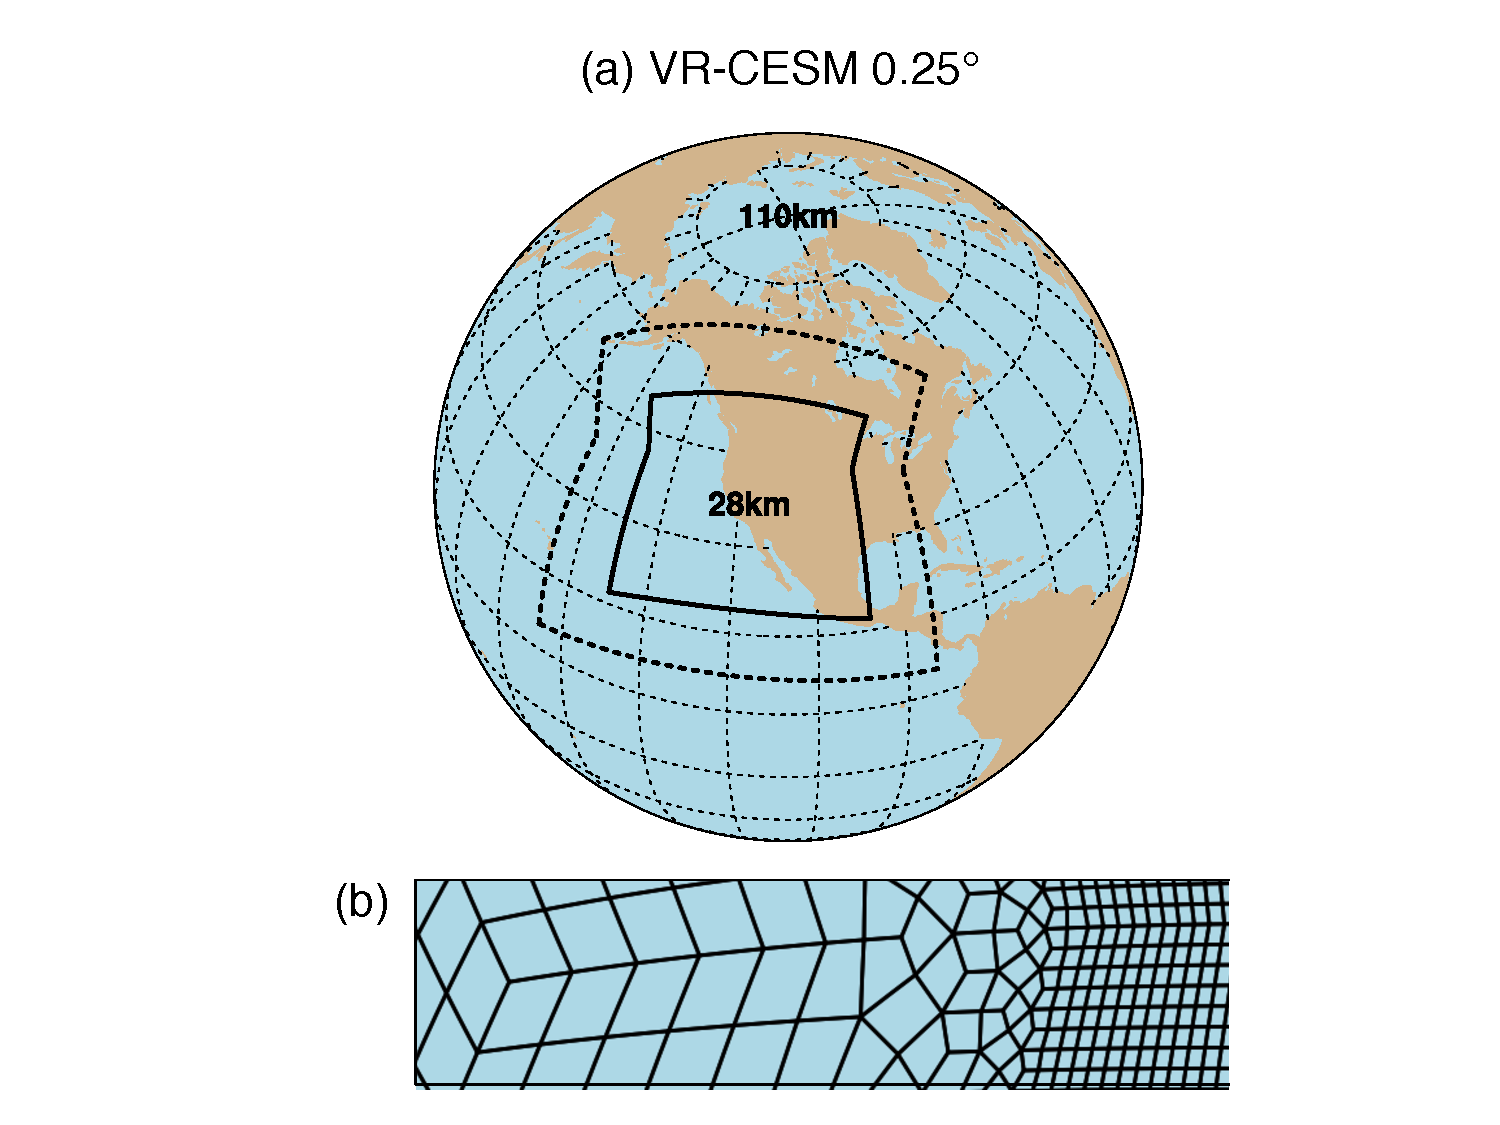
\includegraphics[width=6in]{gridmesh.pdf}
\caption{The approximate grid spacing in the (a) VR-CESM 0.25$^\circ$. (b) A depiction of the transition from the global $1^\circ$ resolution mesh through two layers of refinement to $0.25^\circ$.}
\label{fig:Figure 1}
\end{center}
\end{figure}

\begin{figure}
\begin{center}
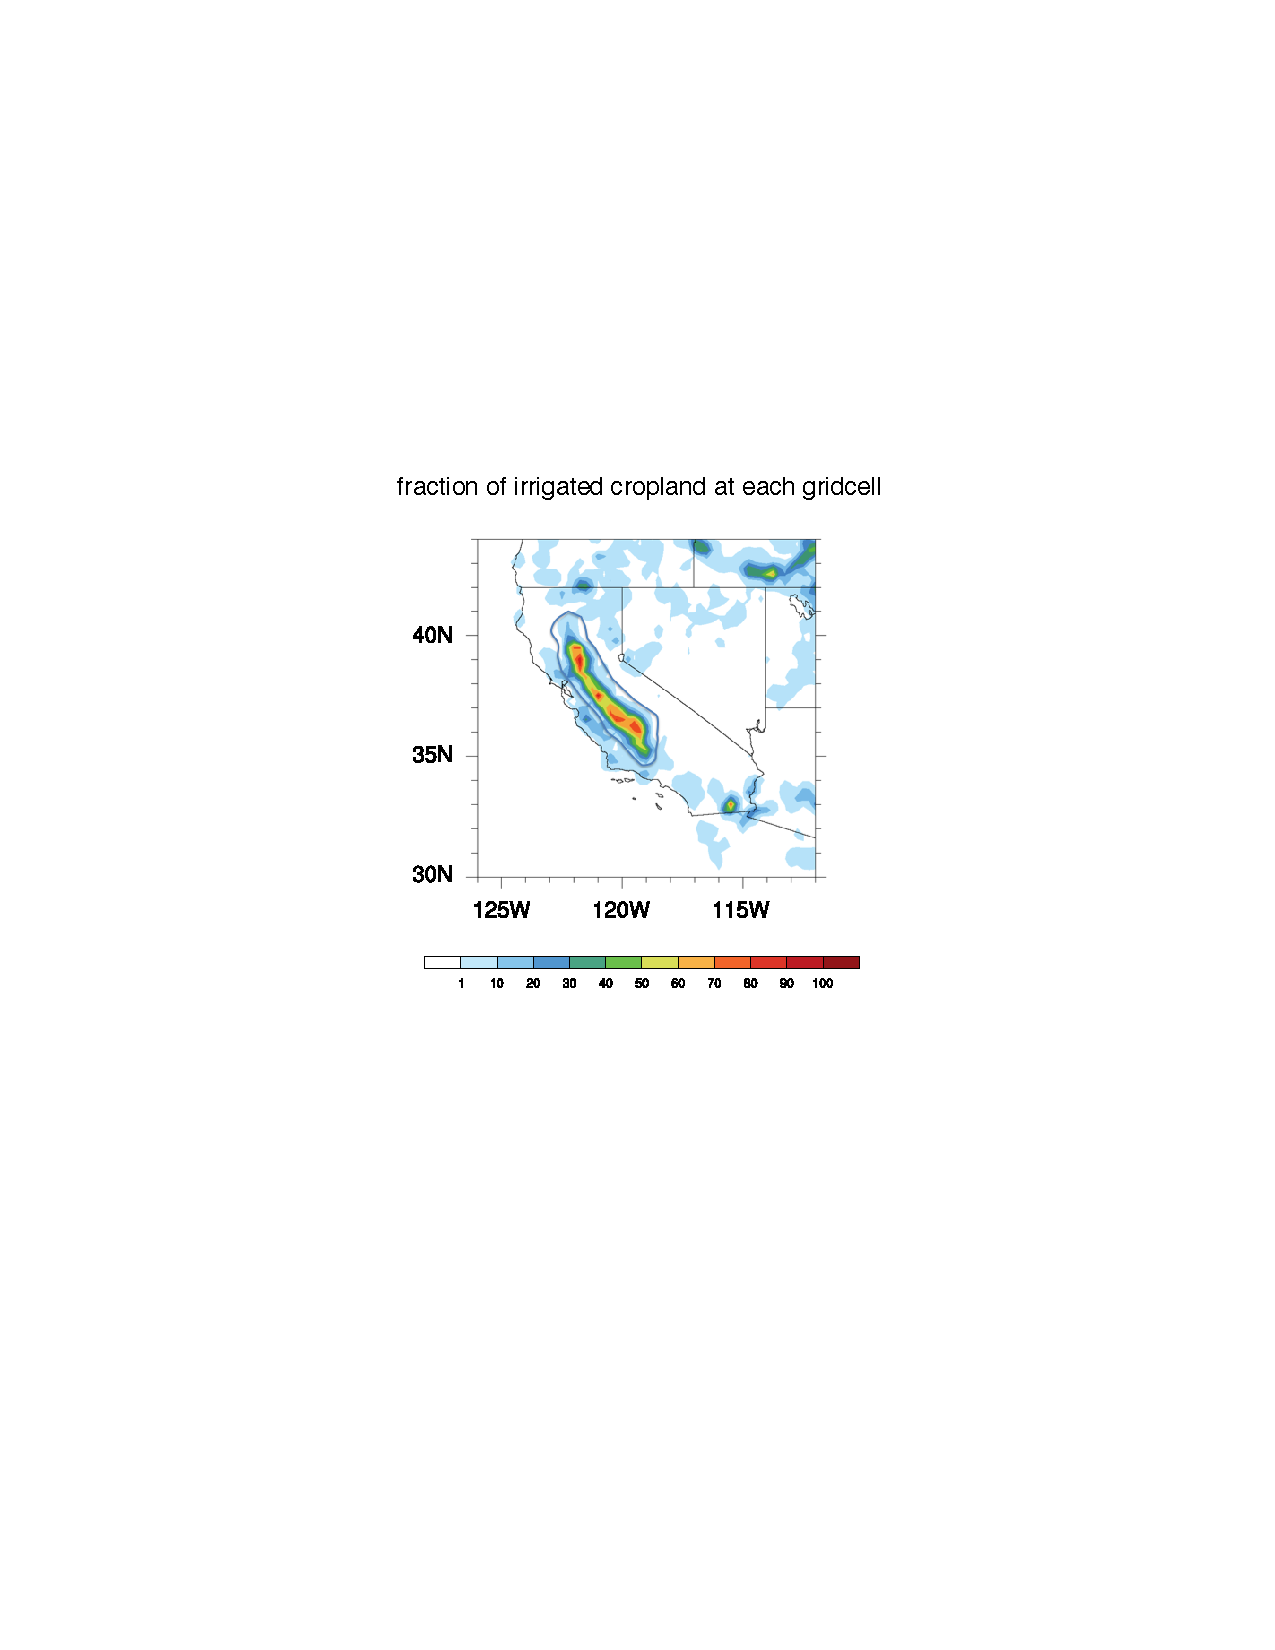
\includegraphics[width=6in]{irrigatedArea.pdf}
\caption{The fraction of irrigated cropland at each grid cell (unit: $\%$) (Blue line is the boundary of the CV region.).}
\label{fig:Figure 2}
\end{center}
\end{figure}

\begin{figure}
\begin{center}
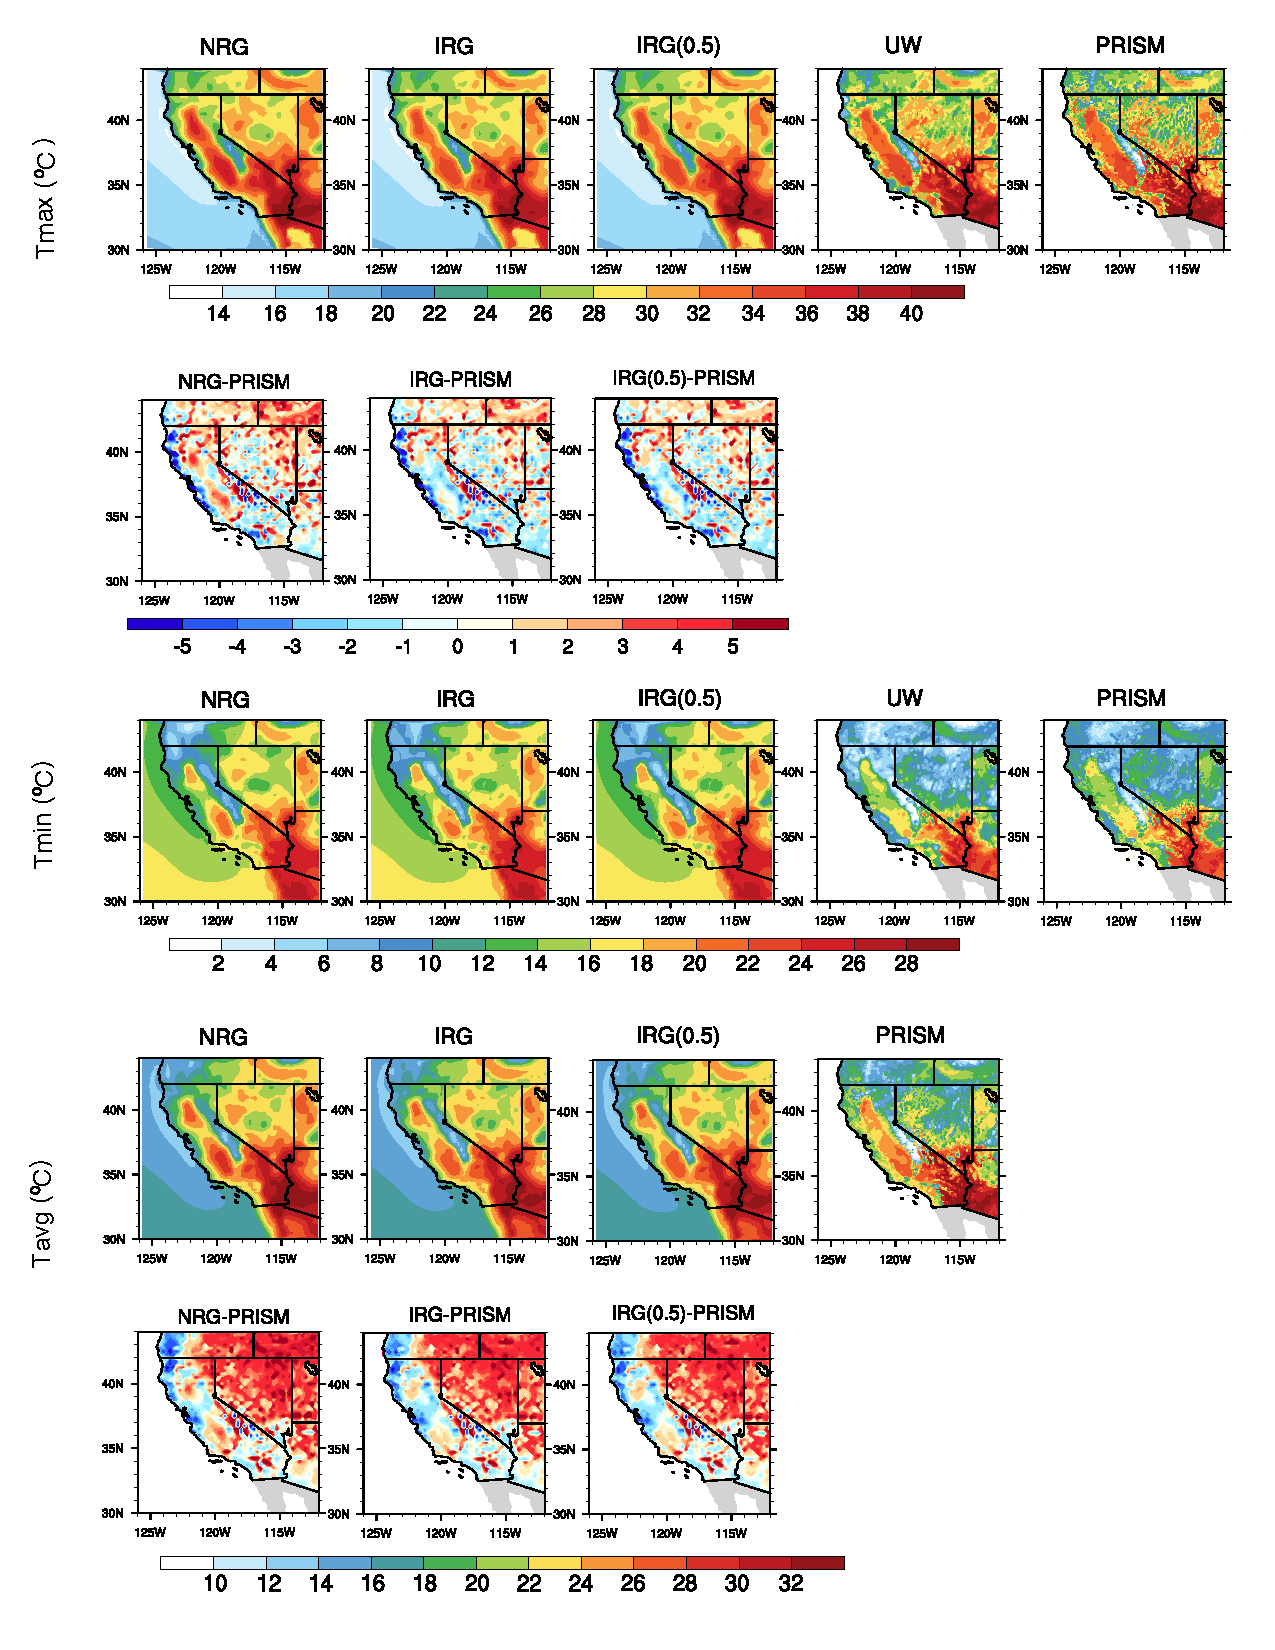
\includegraphics[width=6in]{irrig_2dplot.pdf}
\caption{Average JJA Tmax, Tmin and Tavg over year 1980-2005 for models and observations (unit: $^\circ$C).}
\label{fig:Figure 3}
\end{center}
\end{figure}

\begin{figure}
\begin{center}
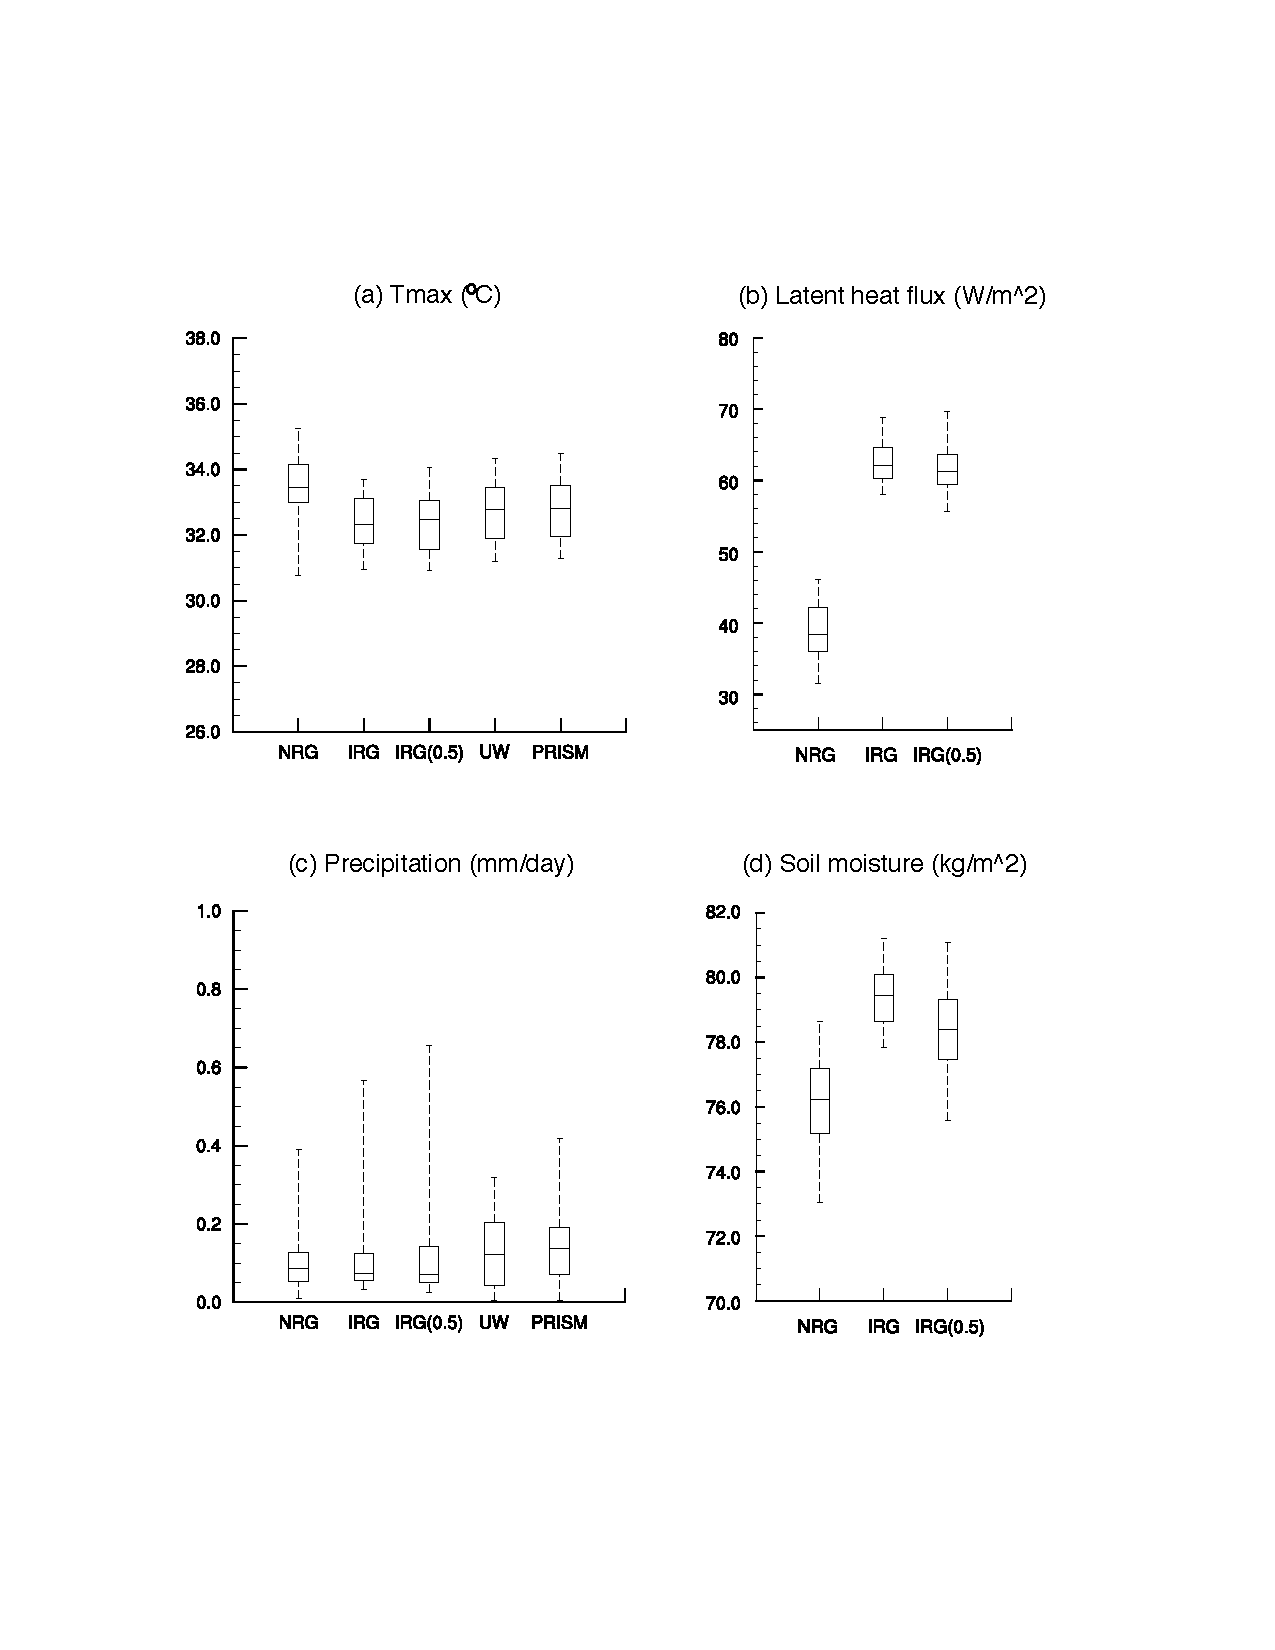
\includegraphics[width=6in]{irrig_boxplot.pdf}
\caption{The boxplot for (a) Tmax, (b) Latent heat flux, (c) Precipitation, and (e) Soil moisture. (From up to down, horizontal lines represent maximum, third quartile, median, first quartile and minimum respectively)} 
\label{fig:Figure 4}
\end{center}
\end{figure}

\begin{figure}
\begin{center}
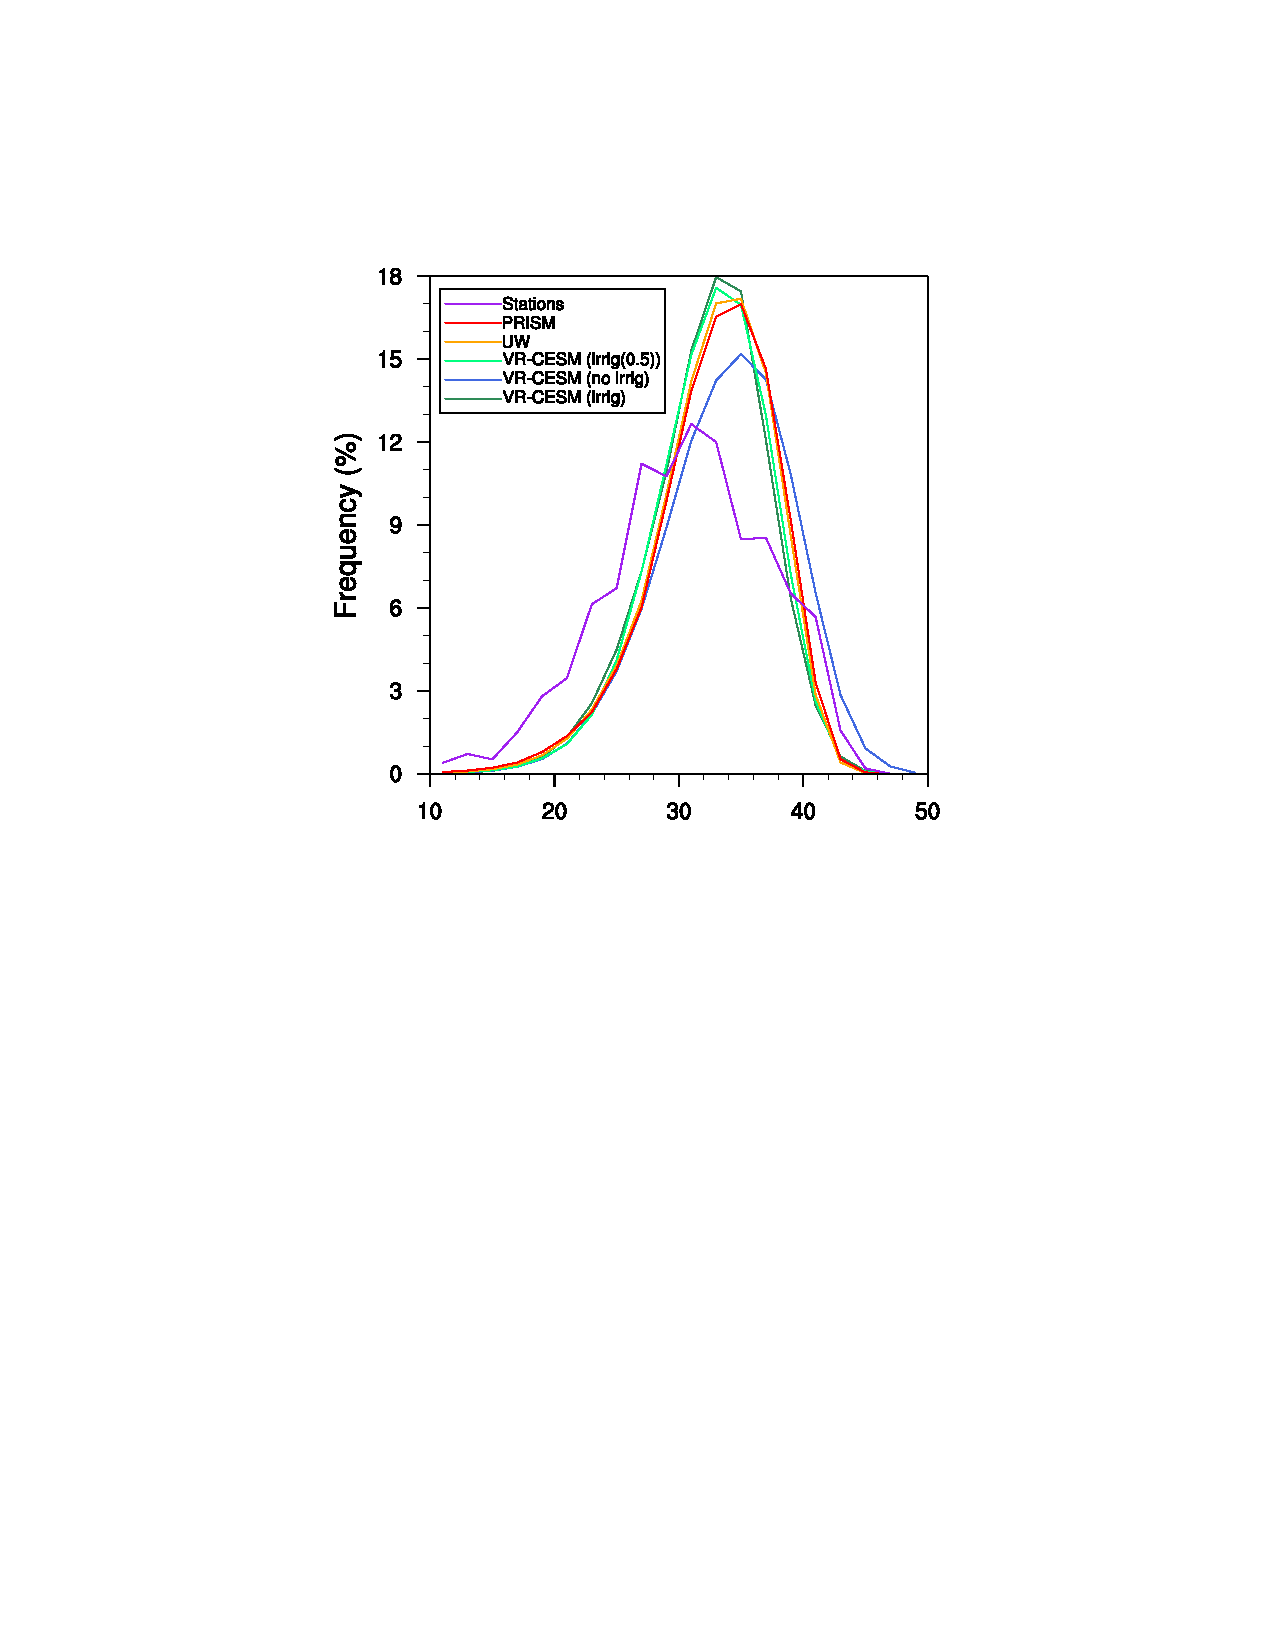
\includegraphics[width=6in]{irrig_pdf_v3.pdf}
\caption{Frequency distribution of JJA daily T$_{max}$ over the simulation period 1981-2005 from simulations and reference datasets.}
\label{fig:Figure 5}
\end{center}
\end{figure}

\begin{figure}
\begin{center}
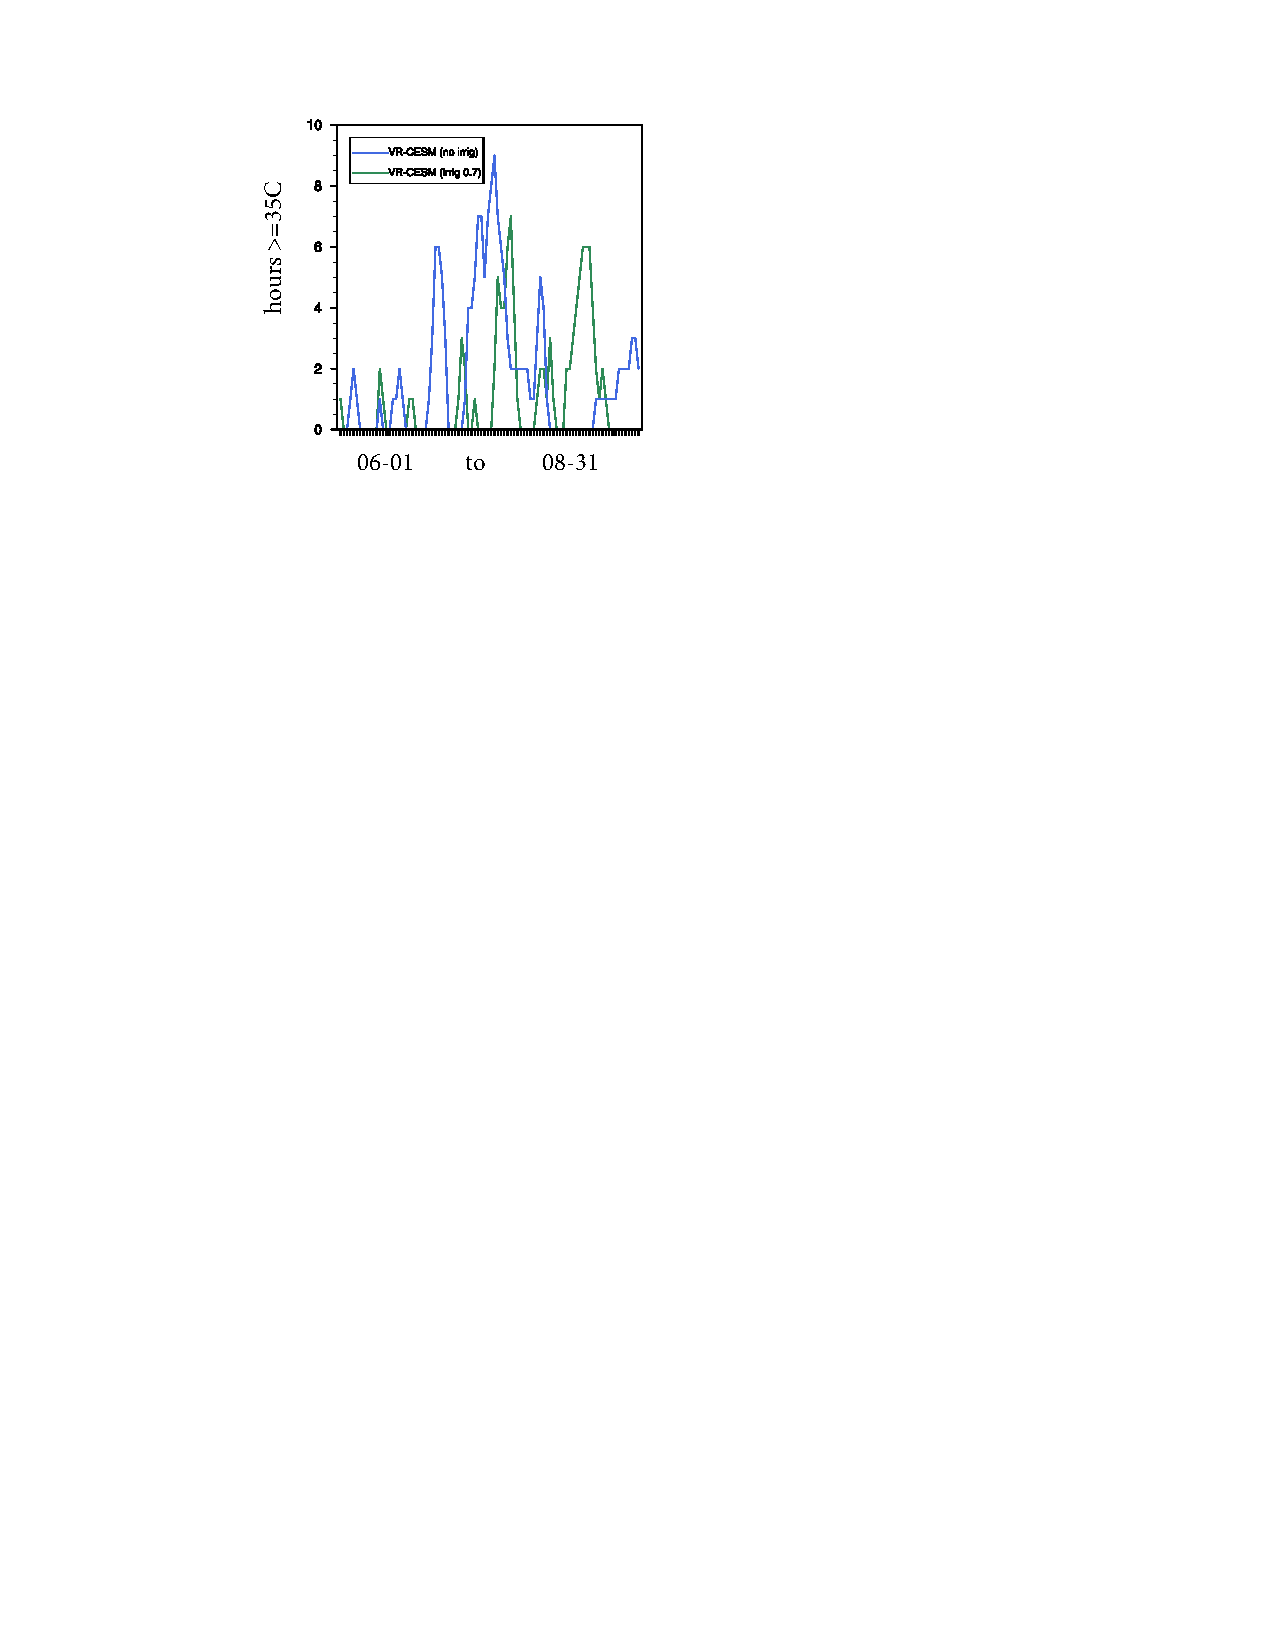
\includegraphics[width=6in]{irrig_hours_T2>=35_v2.pdf}
\caption{The number of hours that larger or equal to 35$^\circ$C per day from June 1st to September (Sept.) 30th averaged over 1980-2005, for NRG and IRG runs.}
\label{fig:Figure 6}
\end{center}
\end{figure}


%\begin{figure}
%\begin{center}
%\includegraphics[width=6in]{irrig_discussion.pdf}
%\caption{.}
%\label{fig:Figure 7}
%\end{center}
%\end{figure}
%change this plot to black and change the legend name

\end{document}